\documentclass[12pt]{book}
\usepackage[a4paper, left=3cm, right=2.5cm, top=2.5cm, bottom=2.5cm]{geometry}

\usepackage[scaled=0.90]{helvet}
\usepackage{microtype}
\usepackage{graphicx}
\usepackage{amsmath, amssymb}
\usepackage{siunitx}
\usepackage{booktabs}
\usepackage{array}
\usepackage{xcolor}
\usepackage[most]{tcolorbox}
\usepackage{float}
\usepackage{tikz}
\usetikzlibrary{arrows.meta, calc, patterns}
\usetikzlibrary{calc}
\usepackage{pgfplots}
\pgfplotsset{compat=1.18}
\usepackage{titlesec}           % must come BEFORE hyperref
\usepackage[colorlinks=true, linkcolor=blue, citecolor=red, urlcolor=purple]{hyperref}
\usepackage{setspace}
\usepackage{fancyhdr}
\usepackage{chngcntr}
\usepackage{enumitem}
\usepackage{microtype}
\usepackage{makecell}
\usepackage{mathrsfs}
\usepackage{caption}


%------Directory Info-------
\graphicspath{{./figures/}}

%------Continuous equation numbering (not reset per chapter)------
\counterwithout{equation}{chapter}

%------Header / Footer------
% No headers on any page; page number centred in the footer only.
\pagestyle{fancy}
\fancyhf{}
\fancyfoot[C]{\thepage}
\renewcommand{\headrulewidth}{0pt}
\renewcommand{\footrulewidth}{0pt}



\fancypagestyle{plain}{%       % chapter-opening pages use "plain" by default
  \fancyhf{}
  \fancyfoot[C]{\thepage}
  \renewcommand{\headrulewidth}{0pt}
  \renewcommand{\footrulewidth}{0pt}
}

%------Custom Box Environments------
\tcbuselibrary{breakable, skins}

% KEY DEFINITION / LAW BOX  — light grey background
\newtcolorbox{keybox}[1][]{
  colback  = gray!10,
  colframe = black!55,
  fonttitle = \bfseries,
  title    = {#1},
  sharp corners,
  boxrule  = 0.5pt,
  left=8pt, right=8pt, top=6pt, bottom=6pt,
  before upper={\setlength{\parskip}{4pt}},
  breakable,
}

% WORKED EXAMPLE BOX  — white background
\newtcolorbox{workedexample}[1][]{
  colback  = white,
  colframe = black!50,
  fonttitle = \bfseries,
  title    = {Worked Example~#1},
  sharp corners,
  boxrule  = 0.5pt,
  left=8pt, right=8pt, top=6pt, bottom=6pt,
  before upper={\setlength{\parskip}{4pt}},
  breakable,
}

% TRY IT YOURSELF BOX  — very light grey
\newtcolorbox{tryit}[1][]{
  colback  = gray!5,
  colframe = black!40,
  fonttitle = \bfseries,
  title    = {Try It Yourself~#1},
  sharp corners,
  boxrule  = 0.5pt,
  left=8pt, right=8pt, top=6pt, bottom=6pt,
  before upper={\setlength{\parskip}{4pt}},
  breakable,
}

% FORMULA SUMMARY BOX  — same shade as keybox
\newtcolorbox{formulabox}[1][Formula Summary]{
  colback  = gray!10,
  colframe = black!55,
  fonttitle = \bfseries,
  title    = {#1},
  sharp corners,
  boxrule  = 0.5pt,
  left=8pt, right=8pt, top=6pt, bottom=6pt,
  before upper={\setlength{\parskip}{4pt}},
  breakable,
}

% STOP AND PREDICT BOX — ISLE-style: an observation or question posed BEFORE
% the physics is revealed. The student should commit to a prediction (write it
% down!) before reading past the box.
\newtcolorbox{predictbox}[1][]{
  colback  = gray!5,
  colframe = black!40,
  fonttitle = \bfseries,
  title    = {Stop and Predict~#1},
  sharp corners,
  boxrule  = 0.5pt,
  leftrule = 3pt,
  left=8pt, right=8pt, top=6pt, bottom=6pt,
  before upper={\setlength{\parskip}{4pt}},
  breakable,
}

% CHECKPOINT BOX — a Mazur-style concept question (ConcepTest). Multiple
% choice, distractors chosen from real student misconceptions. The answer is
% printed upside down via \checkanswer so the eye doesn't grab it first.
\newtcolorbox{checkpoint}[1][]{
  colback  = white,
  colframe = black!55,
  fonttitle = \bfseries,
  title    = {Checkpoint~#1},
  sharp corners,
  boxrule  = 0.5pt,
  toprule  = 2.5pt,
  left=8pt, right=8pt, top=6pt, bottom=6pt,
  before upper={\setlength{\parskip}{4pt}},
  breakable,
}
% Upside-down answer line for checkpoint boxes.
\newcommand{\checkanswer}[1]{%
  \par\smallskip\noindent
  \rotatebox[origin=c]{180}{\parbox{0.93\linewidth}{\scriptsize\itshape #1}}%
}

% SUPPLEMENTARY BOX — enriching but optional. A student in a hurry can skip
% every one of these and still have the full core of the course.
\newtcolorbox{supplementary}[1][]{
  colback  = gray!8,
  colframe = black!40,
  fonttitle = \bfseries,
  title    = {Supplementary --- #1\hfill{\normalfont\footnotesize\itshape optional}},
  sharp corners,
  boxrule  = 0.5pt,
  left=8pt, right=8pt, top=6pt, bottom=6pt,
  before upper={\setlength{\parskip}{4pt}},
  breakable,
}

% WHITEBOARD CHALLENGE BOX — a thinking-classroom group task (after Peter
% Liljedahl's "Building Thinking Classrooms"): done standing at a whiteboard
% or window, in random groups of three, before any solution is shown.
\newtcolorbox{whiteboard}[1][]{
  colback  = white,
  colframe = black!55,
  fonttitle = \bfseries,
  title    = {Whiteboard Challenge~#1\hfill{\normalfont\footnotesize\itshape stand up, groups of three, marker each}},
  sharp corners,
  boxrule  = 1pt,
  left=8pt, right=8pt, top=6pt, bottom=6pt,
  before upper={\setlength{\parskip}{4pt}},
  breakable,
}

%------Chapter Opening Page Design------
% Matches the style in the image:
%   • "CHAPTER" label (small bold) + large grey number — top-right corner
%   • Chapter title — large bold, below
%   • Thick horizontal rule — immediately below the title
%
% For starred chapters (\chapter*) the TikZ overlay is skipped
% automatically (no label block) and only the title + rule appear.

\newlength{\chapboxwd}
\setlength{\chapboxwd}{3.2cm}   % width of the grey number block

\titleformat{\chapter}[display]
  {\normalfont}
  {%
    \begin{tikzpicture}[remember picture, overlay]
      % "CHAPTER" label + plain number, no background box
      \node[anchor=north east, inner sep=0pt, yshift=-42pt]
        at ([xshift=-108pt]current page.north east)
        {\fontsize{15}{15}\selectfont\sffamily\bfseries\MakeUppercase{\chaptertitlename}};
      \node[anchor=north east, inner sep=0pt, yshift=-42pt]
        at ([xshift=-69pt]current page.north east)
        {\fontsize{69}{69}\selectfont\sffamily\bfseries\thechapter};
    \end{tikzpicture}%
  }
  {0pt}
  {%
    \vspace{0.6cm}%   ← tune this to move title up/down
    \Huge\bfseries\sffamily
  }
  [%
    \vspace{-18pt}%
    \noindent\rule{\textwidth}{6pt}%
  ]

\titlespacing*{\chapter}{0pt}{0pt}{12pt}


%------Section and Subsection Headings------
% Section: bold, with a thin underrule (as in the image)
\titleformat{\section}
  {\normalfont\large\sffamily\bfseries}
  {\thesection}
  {1em}
  {}
  [\vspace{-15pt}\rule{\textwidth}{1pt}]

\titlespacing*{\section}{0pt}{15pt}{3pt}

% --- Custom Colors ---
\definecolor{paper}{HTML}{F2E4C2}
\definecolor{accentblue}{HTML}{1F6FB2}
\definecolor{accentred}{HTML}{C0392B}
\definecolor{skintone}{HTML}{FCDCB6}
\definecolor{skinoutline}{HTML}{D29864}
\definecolor{myblue}{HTML}{2E86C1}
\definecolor{myred}{HTML}{C0392B}
\definecolor{mygreen}{HTML}{1E8449}
\definecolor{myorange}{HTML}{D35400}




\titleformat{\subsection}
  {\normalfont\normalsize\sffamily\bfseries}
  {}      % ← empty label = no number
  {0em}
  {}

\titlespacing*{\subsection}{0pt}{14pt}{4pt}


%removing subsection from TOC
\setcounter{tocdepth}{1}


%------Formatting------
\setlength\parindent{0pt}
\setlength\parskip{6pt}
\renewcommand{\arraystretch}{1.3}

%------Title Page------
\title{%
  {\sffamily \Huge \bfseries Fundamentals of Physics}
}

\vspace{6cm}

\author{%
  \sffamily Tashi Wangchuk\\
  \normalsize Druk Gyalpo's Institute, Pangbisa, Paro 12001, Bhutan \\[-0.5em]
  \href{mailto:tashiwangchuk@academy.bt}{\texttt{\small tashiwangchuk@academy.bt}}%
}
\date{\normalsize April 2026}


\begin{document}
\frontmatter
\maketitle

%%-------------Acknowledgements-----------------
\chapter*{Acknowledgements}
\addcontentsline{toc}{chapter}{Acknowledgements}

These lecture notes are anything but original. My main contribution has been to gather,
adapt, and weave together the clearest discussions and explanations I could find in the vast
literature on the subject. The lectures lean heavily on the sources listed in the syllabus, and
much of the brainstorming was done in conversation with Claude AI.

\vspace{0.3cm}

I thank my students, whose evident grasp of the material has shown me where to simplify
and where to linger in detail. I am supported by the Druk Gyalpo's Institute.


%%-----------Table of Contents------------------
\renewcommand{\contentsname}{Table of Contents}
\clearpage
\addcontentsline{toc}{chapter}{Table of Contents}
\tableofcontents

%%-------------Begin Main Matter-----------------
\clearpage
\mainmatter

%%-----------Chapter 1------------------------------------------
\chapter{Vectors}

\section{Introduction to Scalars and Vectors}

Imagine you walk from corner A to corner C (a distance of 4\,m), then turn and walk from
C to B (a distance of 3\,m).
\begin{itemize}
  \item The total \emph{distance} you walked is $4+3=7$\,m. Distance only cares about how much, not which way.
  \item Your \emph{displacement} --- the straight-line shortcut from start to finish --- is only 5\,m, pointing from A to B. Displacement cares about how much \emph{and} which way.
\end{itemize}

\begin{keybox}[Scalars and Vectors]
A \textbf{scalar} is a quantity that has magnitude only (no direction): distance, mass, time, temperature, speed, energy.

A \textbf{vector} is a quantity that has magnitude and direction: displacement, velocity, acceleration, force.
\end{keybox}

\begin{center}
\begin{tabular}{lcc}
  \toprule
               & \textbf{Scalar} & \textbf{Vector} \\
  \midrule
  Has magnitude & yes & yes \\
  Has direction & no  & yes \\
  Examples & distance, speed, mass, time & displacement, velocity, force \\
  \bottomrule
\end{tabular}
\end{center}

\subsection{Notation}
\begin{itemize}
  \item Vectors are written with a small arrow above the symbol, e.g.\ a force $\vec{F}$ or a velocity $\vec{v}$.
  \item The magnitude (size) of a vector $\vec{A}$ is written $|\vec{A}|$, or simply $A$.
  \item In diagrams a vector is drawn as an arrow: the length of the arrow is proportional to the magnitude, and the arrowhead shows the direction.
\end{itemize}

\begin{keybox}[Vectors have magnitude and direction, but not location]
A displacement of 1\,m due east from Paro is represented by the \emph{same} vector as a
displacement of 1\,m due east from Thimphu. Sliding a vector to a new position (without
rotating or resizing it) does not change the vector at all.
\end{keybox}

\subsection{The negative of a vector}
$-\vec{A}$ is a vector with the same magnitude as $\vec{A}$ but pointing in the opposite direction.


\section{Vector Operations}

\subsection{Addition of vectors (head-to-tail / triangle rule)}
To add two vectors, place the tail of $\vec{B}$ at the head of $\vec{A}$. The sum $\vec{A}+\vec{B}$ is
the vector drawn from the tail of $\vec{A}$ to the head of $\vec{B}$. This sum is called the
\textbf{resultant vector}.

Addition is \textbf{commutative}: $\vec{A}+\vec{B} = \vec{B}+\vec{A}$.

Addition is \textbf{associative}: $(\vec{A}+\vec{B})+\vec{C} = \vec{A}+(\vec{B}+\vec{C})$.

Subtraction means adding the opposite: $\vec{A}-\vec{B} = \vec{A}+(-\vec{B})$.

\subsection{Parallelogram law of vector addition}
Draw $\vec{a}$ and $\vec{b}$ with both tails together. Treat them as two adjacent sides and
complete the parallelogram. The diagonal through the common tails is the sum $\vec{a}+\vec{b}=\vec{R}$.

\textbf{Deriving the magnitude and direction of the resultant.}
Let $a=|\vec{a}|$, $b=|\vec{b}|$, and let $\theta$ be the angle between them. By the law of cosines
applied to the triangle formed:
\begin{align}
  R^2 &= a^2 + 2ab\cos\theta + b^2, \notag
\end{align}
so

\begin{keybox}[Magnitude and direction of the resultant]
\[
  R = |\vec{a}+\vec{b}| = \sqrt{a^2 + 2ab\cos\theta + b^2}
\]
\[
  \alpha = \tan^{-1}\!\left(\frac{b\sin\theta}{a+b\cos\theta}\right)
  \qquad \text{(angle that $\vec{R}$ makes with $\vec{a}$)}
\]
\end{keybox}

\begin{workedexample}[1.1: Resultant of two forces]
Two forces of $a=3$\,N and $b=4$\,N act at a point with an angle of $\theta=60^\circ$ between
them. Find the magnitude and direction of the resultant.

\medskip
\textit{Solution.}
\[
  R = \sqrt{3^2 + 2(3)(4)\cos60^\circ + 4^2} = \sqrt{9+12+16} = \sqrt{37} \approx 6.1\;\text{N}.
\]
\[
  \alpha = \tan^{-1}\!\left(\frac{4\sin60^\circ}{3+4\cos60^\circ}\right)
         = \tan^{-1}\!\left(\frac{3.46}{5}\right) \approx 34.7^\circ
\]
measured from the 3\,N force.
\end{workedexample}

\begin{tryit}[1.1: Two velocities]
A boat heads north at $a=6$\,m/s while a current pushes it at $b=8$\,m/s at $\theta=90^\circ$
to the boat's heading. Show that the resultant speed is 10\,m/s and find its direction
relative to north.
\end{tryit}

\subsection{Multiplication by a scalar}
Multiplying a vector by a positive scalar $n$ multiplies its magnitude but leaves the direction
unchanged. If $n$ is negative, the direction is reversed. Scalar multiplication is distributive:
\[
  n(\vec{A}+\vec{B}) = n\vec{A}+n\vec{B}.
\]

\subsection{The dot (scalar) product}

\begin{keybox}[Dot product]
\[
  \vec{A}\cdot\vec{B} \equiv AB\cos\theta,
\]
where $\theta$ is the angle between the vectors when placed tail to tail. The result is a
scalar --- hence the alternative name \emph{scalar product}.
\end{keybox}

Geometrically, $\vec{A}\cdot\vec{B}$ is the magnitude of $\vec{A}$ times the projection of $\vec{B}$
along $\vec{A}$ (which is $B\cos\theta$), or equivalently $B$ times the projection of $\vec{A}$ along $\vec{B}$.

\textbf{Properties.}
\begin{itemize}
  \item Commutative: $\vec{A}\cdot\vec{B}=\vec{B}\cdot\vec{A}$.
  \item Distributive: $\vec{A}\cdot(\vec{B}+\vec{C})=\vec{A}\cdot\vec{B}+\vec{A}\cdot\vec{C}$.
  \item A vector dotted with itself gives its magnitude squared: $\vec{A}\cdot\vec{A}=A^2$.
  \item If $\vec{A}\perp\vec{B}$, then $\vec{A}\cdot\vec{B}=AB\cos90^\circ=0$.
\end{itemize}

\begin{workedexample}[1.2: Work done by a force]
A force $\vec{F}$ of magnitude 10\,N acts at $30^\circ$ to a displacement $\vec{d}$ of magnitude 5\,m.
The work done is $W=\vec{F}\cdot\vec{d}$:
\[
  W = Fd\cos\theta = (10)(5)\cos30^\circ \approx 43.3\;\text{J}.
\]
\end{workedexample}

\begin{workedexample}[1.3: Class exercise --- the Law of Cosines]
Let $\vec{C}=\vec{A}-\vec{B}$. Calculate the dot product of $\vec{C}$ with itself.

\medskip
\textit{Solution.}
\begin{align*}
  \vec{C}\cdot\vec{C} &= (\vec{A}-\vec{B})\cdot(\vec{A}-\vec{B})
  = \vec{A}\cdot\vec{A} - \vec{A}\cdot\vec{B} - \vec{B}\cdot\vec{A} + \vec{B}\cdot\vec{B}\\
  &= A^2 - AB\cos\theta - BA\cos\theta + B^2.
\end{align*}
\[
  \boxed{C^2 = A^2 + B^2 - 2AB\cos\theta} \qquad\text{(the Law of Cosines).}
\]
\end{workedexample}

\subsection{The cross (vector) product}

\begin{keybox}[Cross product]
\[
  \vec{A}\times\vec{B} \equiv AB\sin\theta\;\hat{n},
\]
where $\hat{n}$ is a unit vector pointing perpendicular to the plane containing $\vec{A}$ and
$\vec{B}$. The result is itself a vector --- hence the name \emph{vector product}.
\end{keybox}

The magnitude is $|\vec{A}\times\vec{B}|=AB\sin\theta$.

\begin{keybox}[Right-hand rule]
Point the fingers of your right hand along the first vector, curl them through the smaller
angle toward the second vector --- your thumb then points along $\hat{n}$.
\end{keybox}

\textbf{Properties.}
\begin{itemize}
  \item Distributive: $\vec{A}\times(\vec{B}+\vec{C})=\vec{A}\times\vec{B}+\vec{A}\times\vec{C}$.
  \item \textbf{Not commutative} --- order matters: $\vec{B}\times\vec{A}=-(\vec{A}\times\vec{B})$.
  \item Geometrically, $|\vec{A}\times\vec{B}|$ equals the area of the parallelogram with sides $\vec{A}$ and $\vec{B}$.
  \item Parallel vectors give zero: $\vec{A}\times\vec{A}=A^2\sin0^\circ\,\hat{n}=\vec{0}$.
\end{itemize}

\begin{workedexample}[1.4: Torque]
A spanner is turned by a force $F=20$\,N applied at the end of a handle of length $r=0.30$\,m,
at $90^\circ$ to the handle. The torque magnitude is
\[
  |\vec{\tau}| = |\vec{r}\times\vec{F}| = rF\sin90^\circ = (0.30)(20)(1) = 6\;\text{N\,m}.
\]
\end{workedexample}


\section{Components of a Vector}

It is often useful to describe a vector in terms of its components. If a vector $\vec{A}$ is split
into two mutually perpendicular vectors, these are called the \textbf{rectangular components}
of $\vec{A}$.

The vector $\vec{A}$ has magnitude $A$ and makes angle $\theta$ with the positive $x$-axis.

\begin{keybox}[Finding the components from magnitude and angle]
\[
  A_x = A\cos\theta, \qquad A_y = A\sin\theta.
\]
\end{keybox}

We can reverse the process to recover the magnitude and direction:
\[
  A_x^2 + A_y^2 = A^2(\cos^2\theta+\sin^2\theta) = A^2, \qquad
  \frac{A_y}{A_x} = \tan\theta.
\]

\begin{keybox}[Finding magnitude and angle from the components]
\[
  A = \sqrt{A_x^2+A_y^2}, \qquad \theta = \tan^{-1}\!\left(\frac{A_y}{A_x}\right).
\]
\end{keybox}

\begin{workedexample}[1.5: Resolving a force]
A force of $A=100$\,N acts at $\theta=30^\circ$ above the horizontal. Its components are
\[
  A_x = 100\cos30^\circ \approx 86.6\;\text{N}, \qquad A_y = 100\sin30^\circ = 50\;\text{N}.
\]
\end{workedexample}

\begin{workedexample}[1.6: Adding vectors using components]
Add $\vec{A}$ (5\,m at $37^\circ$) and $\vec{B}$ (8\,m at $0^\circ$, i.e.\ along $x$).

\medskip
\textit{Solution.} Resolve each, add like components, then recombine.
\begin{align*}
  A_x &= 5\cos37^\circ \approx 4.0, & A_y &= 5\sin37^\circ \approx 3.0,\\
  B_x &= 8,                          & B_y &= 0.
\end{align*}
\[
  R_x = 4.0+8 = 12.0, \qquad R_y = 3.0+0 = 3.0.
\]
\[
  R = \sqrt{12.0^2+3.0^2} \approx 12.4\;\text{m}, \qquad
  \theta = \tan^{-1}\!\!\left(\frac{3.0}{12.0}\right) \approx 14^\circ.
\]
\end{workedexample}

\begin{tryit}[1.2: Components of velocity]
A projectile is launched at 20\,m/s, $60^\circ$ above the horizontal. Find the horizontal and
vertical components of the launch velocity.

\textit{(Answer: $v_x=10$\,m/s, $v_y\approx17.3$\,m/s.)}
\end{tryit}


\section{Vector Algebra in Components}

In practice it is often easiest to set up Cartesian coordinates $x,y,z$ and work with
components.

\subsection{Basis vectors and unit vectors}
Let $\hat{x},\hat{y},\hat{z}$ (sometimes written $\hat{\imath},\hat{\jmath},\hat{k}$) be unit vectors
pointing along the $x$-, $y$-, and $z$-axes. These are the \textbf{basis vectors}.

\begin{keybox}[Unit vector]
A unit vector has magnitude exactly 1; its only job is to indicate direction. Any vector
$\vec{A}$ can be turned into a unit vector (written $\hat{A}$) by dividing by its own magnitude:
\[
  \hat{A} = \frac{\vec{A}}{|\vec{A}|}.
\]
\end{keybox}

\subsection{Component form of a vector}
Any vector can be written in terms of the basis vectors:
\[
  \vec{A} = A_x\hat{x} + A_y\hat{y} + A_z\hat{z}.
\]
The coefficients $A_x,A_y,A_z$ are the \emph{components} of $\vec{A}$ --- geometrically, the
projections of $\vec{A}$ onto the three axes. A component can be extracted by dotting with
the matching basis vector:
\[
  \vec{A}\cdot\hat{x} = A_x, \qquad \vec{A}\cdot\hat{y} = A_y, \qquad \vec{A}\cdot\hat{z} = A_z.
\]

\subsection{The four operations in component form}

\begin{keybox}[Rule 1 --- Addition: add like components]
\[
  \vec{A}+\vec{B} = (A_x+B_x)\hat{x} + (A_y+B_y)\hat{y} + (A_z+B_z)\hat{z}
\]
\end{keybox}

\begin{keybox}[Rule 2 --- Scalar multiplication: scale every component]
\[
  a\vec{A} = (aA_x)\hat{x} + (aA_y)\hat{y} + (aA_z)\hat{z}
\]
\end{keybox}

\begin{keybox}[Rule 3 --- Dot product: multiply like components and add]
\[
  \vec{A}\cdot\vec{B} = A_xB_x + A_yB_y + A_zB_z
\]
\end{keybox}

This works because the basis vectors are mutually perpendicular unit vectors:
\[
  \hat{x}\cdot\hat{x}=\hat{y}\cdot\hat{y}=\hat{z}\cdot\hat{z}=1, \qquad
  \hat{x}\cdot\hat{y}=\hat{x}\cdot\hat{z}=\hat{y}\cdot\hat{z}=0.
\]
In particular $\vec{A}\cdot\vec{A}=A_x^2+A_y^2+A_z^2$, so

\begin{keybox}[Magnitude (3-D Pythagoras)]
\[
  |\vec{A}| = \sqrt{A_x^2+A_y^2+A_z^2}
\]
\end{keybox}

\begin{keybox}[Bonus --- Rule 4: the cross product as a determinant]
\[
  \vec{A}\times\vec{B} = \begin{vmatrix}\hat{x}&\hat{y}&\hat{z}\\A_x&A_y&A_z\\B_x&B_y&B_z\end{vmatrix}
  = (A_yB_z-A_zB_y)\hat{x} - (A_xB_z-A_zB_x)\hat{y} + (A_xB_y-A_yB_x)\hat{z}
\]
\end{keybox}

\begin{workedexample}[1.7: Putting the rules together]
Let $\vec{A}=2\hat{x}+3\hat{y}+\hat{z}$ and $\vec{B}=\hat{x}-\hat{y}+4\hat{z}$.

\medskip
(a) \textit{Sum.} $\vec{A}+\vec{B}=(2+1)\hat{x}+(3-1)\hat{y}+(1+4)\hat{z}=3\hat{x}+2\hat{y}+5\hat{z}$.

(b) \textit{Dot product.} $\vec{A}\cdot\vec{B}=(2)(1)+(3)(-1)+(1)(4)=2-3+4=3$.

(c) \textit{Magnitude of $\vec{A}$.} $|\vec{A}|=\sqrt{2^2+3^2+1^2}=\sqrt{14}\approx3.74$.

(d) \textit{Angle between them.} Using $\vec{A}\cdot\vec{B}=AB\cos\theta$ with $|\vec{B}|=\sqrt{1+1+16}=\sqrt{18}$:
\[
  \cos\theta = \frac{3}{\sqrt{14}\,\sqrt{18}} \approx 0.189 \implies \theta \approx 79^\circ.
\]
\end{workedexample}


\section{Position, Displacement, and Separation Vectors}

\subsection{Position vector}
A point in space is described by its Cartesian coordinates: $(x,y)$ in 2-D or $(x,y,z)$ in
3-D. The vector from the origin $O$ to that point is the \textbf{position vector}:
\[
  \vec{r} \equiv x\hat{x}+y\hat{y}+z\hat{z}.
\]
Its magnitude is the distance from the origin, $r=\sqrt{x^2+y^2+z^2}$, and the unit vector
pointing radially outward is
\[
  \hat{r} = \frac{\vec{r}}{r} = \frac{x\hat{x}+y\hat{y}+z\hat{z}}{\sqrt{x^2+y^2+z^2}}.
\]

\subsection{Separation vector}

\begin{keybox}[Separation vector $\vec{\Delta}$]
The separation vector is the displacement from a source point $\vec{r}\,'$ (where something
is located, e.g.\ an electric charge) to a field point $\vec{r}$ (where you are observing):
\[
  \vec{\Delta} \equiv \vec{r}-\vec{r}\,'.
\]
\end{keybox}

Its magnitude is $\Delta=|\vec{r}-\vec{r}\,'|$, and the unit vector pointing from the source to the
field point is
\[
  \hat{\Delta} = \frac{\vec{\Delta}}{\Delta} = \frac{\vec{r}-\vec{r}\,'}{|\vec{r}-\vec{r}\,'|}.
\]
In Cartesian coordinates,
\begin{align*}
  \vec{\Delta} &= (x-x')\hat{x}+(y-y')\hat{y}+(z-z')\hat{z},\\
  \Delta &= \sqrt{(x-x')^2+(y-y')^2+(z-z')^2},\\
  \hat{\Delta} &= \frac{(x-x')\hat{x}+(y-y')\hat{y}+(z-z')\hat{z}}{\sqrt{(x-x')^2+(y-y')^2+(z-z')^2}}.
\end{align*}

\begin{workedexample}[1.8: A separation vector]
A charge sits at the source point $\vec{r}\,'=(1,0,2)$ and we observe at the field point
$\vec{r}=(4,4,2)$ (coordinates in metres). Then
\[
  \vec{\Delta} = (4-1)\hat{x}+(4-0)\hat{y}+(2-2)\hat{z} = 3\hat{x}+4\hat{y},
\]
\[
  \Delta = \sqrt{3^2+4^2+0^2} = 5\;\text{m}, \qquad
  \hat{\Delta} = \tfrac{3}{5}\hat{x}+\tfrac{4}{5}\hat{y}.
\]
\end{workedexample}

\begin{keybox}[When are two vectors equal?]
Two vectors are equal only if their corresponding components are equal --- equivalently,
if they have the same magnitude and the same direction. Sliding a vector to a new position
(a parallel translation) does not change it.
\end{keybox}


\section*{Formula Summary: Vectors}
\addcontentsline{toc}{section}{Formula Summary: Vectors}

\begin{formulabox}[Formula Summary: Vectors]
\begin{tabular}{ll}
  \toprule
  \textbf{Quantity} & \textbf{Formula} \\
  \midrule
  Resultant (parallelogram law) & $R=\sqrt{a^2+2ab\cos\theta+b^2}$ \\[4pt]
  Direction of resultant & $\alpha=\tan^{-1}\!\bigl(\tfrac{b\sin\theta}{a+b\cos\theta}\bigr)$ \\[4pt]
  Dot product & $\vec{A}\cdot\vec{B}=AB\cos\theta=A_xB_x+A_yB_y+A_zB_z$ \\[4pt]
  Cross-product magnitude & $|\vec{A}\times\vec{B}|=AB\sin\theta$ \\[4pt]
  Components (2-D) & $A_x=A\cos\theta$,\quad $A_y=A\sin\theta$ \\[4pt]
  Magnitude (2-D) & $A=\sqrt{A_x^2+A_y^2}$ \\[4pt]
  Magnitude (3-D) & $A=\sqrt{A_x^2+A_y^2+A_z^2}$ \\[4pt]
  Unit vector & $\hat{A}=\vec{A}/|\vec{A}|$ \\[4pt]
  Position vector & $\vec{r}=x\hat{x}+y\hat{y}+z\hat{z}$ \\[4pt]
  Separation vector & $\vec{\Delta}=\vec{r}-\vec{r}\,'$ \\
  \bottomrule
\end{tabular}
\end{formulabox}

%%-----------Chapter 2------------------------------------------
\chapter{Dimensional Analysis}

Here is a challenge that sounds impossible. Take a pendulum --- a stone on a
string. Its period (the time for one full swing) surely depends on things like
the length of the string, the mass of the stone, how hard gravity pulls. Now
the challenge: \emph{predict the formula for the period without using any law
of motion at all}. No forces, no Newton, no experiment. Just bookkeeping.

By the end of this short chapter you will do exactly that --- and you will
discover along the way that the mass of the stone \emph{cannot appear in the
answer}, a fact you can then walk outside and test with two stones and a
shoelace. The trick is called \textbf{dimensional analysis}, and physicists
reach for it constantly: to catch algebra mistakes, to guess formulas before
deriving them, and sometimes (as the supplementary box at the end of the
chapter shows) to uncover military secrets from a published photograph.

\begin{predictbox}[2.1: The pendulum, before any theory]
A pendulum of length $l$ carries a bob of mass $m$, swinging under gravity
$g$. Before reading on, write down your instincts:
\begin{enumerate}[leftmargin=2em, itemsep=1pt]
  \item If you double the mass of the bob, does the period get longer,
        shorter, or stay the same?
  \item If you double the length of the string, what happens to the period ---
        doubles? quadruples? something else?
\end{enumerate}
Keep your answers. The chapter will grade them --- twice: once by bookkeeping,
once (if your class has a shoelace) by experiment.
\end{predictbox}

\section{Dimension}

In physics, we measure many different things, but they are all built from a small set of seven
fundamental base quantities (see Table~\ref{tab:base_quantities}).

\begin{table}[H]
  \centering
  \caption{The seven fundamental base quantities, their dimensions, and sample units.}
  \label{tab:base_quantities}
  \begin{tabular}{lcc}
    \toprule
    \textbf{Base Quantity} & \textbf{Dimension} & \textbf{Sample Units} \\
    \midrule
    Mass                          & $[M]$     & kg, g, lbs \\
    Length                        & $[L]$     & m, cm, feet, miles \\
    Time                          & $[T]$     & s, minutes, hours, years \\
    Electric Current              & $[I]$     & A, mA \\
    Thermodynamic Temperature     & $[\Theta]$& K, $^\circ$C, $^\circ$F \\
    Amount of Substance           & $[N]$     & mol \\
    Luminous Intensity            & $[J]$     & cd \\
    \bottomrule
  \end{tabular}
\end{table}

The \textbf{dimension} of any physical quantity represents the powers to which these base
quantities must be raised to express that quantity. Example:
\[
  [\text{Force}] = [\text{mass}]\times\frac{[\text{velocity}]}{[\text{time}]}
                 = [\text{mass}]\times\frac{[\text{length/time}]}{[\text{time}]}
                 = MLT^{-2}.
\]
Such an expression for a physical quantity in terms of the base quantities is called the
\textbf{dimensional formula}. Thus, the dimensional formula of force is $MLT^{-2}$. In other
words, we say the dimensions of force are 1 in mass, 1 in length, and $-2$ in time. The
dimensions in all other base quantities are zero.

Note that in this type of calculation the magnitudes are not considered. It is equality of the
\emph{type} of quantity that enters. Thus, change in velocity, initial velocity, average velocity,
and final velocity are all equivalent in this discussion --- each one is $LT^{-1}$.

The physical quantity that is expressed in terms of the base quantities is enclosed in square
brackets to remind us that the equation is among the dimensions and not among the magnitudes.


\section{The Principle of Homogeneity}

You cannot add apples to oranges, and in physics, you cannot add velocity to force.

\begin{keybox}[The Principle of Homogeneity]
The dimensions of all separated terms in a physical equation must be identical.
\end{keybox}

Let us check the kinematic equation $x = ut + \tfrac{1}{2}at^2$:
\begin{itemize}
  \item $[x] = L$
  \item $[ut] = (LT^{-1})(T) = L$
  \item $[\tfrac{1}{2}at^2] = (LT^{-2})(T^2) = L$
\end{itemize}
Since every term evaluates to length $[L]$, the equation is dimensionally correct. Note: the
constant $\tfrac{1}{2}$ has no dimension and is ignored in this check.

\begin{checkpoint}[2.1: Spot the impostor]
A student solving a problem about a falling stone produces four candidate
formulas, where $v$ is a speed, $g$ an acceleration, $h$ a height, and $t$ a
time. Exactly one of them \emph{could} be right. Which one?
\begin{enumerate}[label=(\alph*), leftmargin=2.5em, itemsep=0pt]
  \item $v = 2gh$
  \item $v = \sqrt{2gh}$
  \item $h = \tfrac12 g t$
  \item $t = \sqrt{2h g}$
\end{enumerate}
\checkanswer{Answer: (b). Check each: $[gh]=(LT^{-2})(L)=L^2T^{-2}$, which is
speed \emph{squared} --- so (a) fails but its square root (b) has dimension
$LT^{-1}$, a speed. In (c), $[gt]=LT^{-1}$ is a speed, not a height. In (d),
$[\sqrt{hg}]=\sqrt{L^2T^{-2}}=LT^{-1}$, again a speed, not a time. Note what
the check cannot do: it cannot tell you whether the 2 in (b) is right.}
\end{checkpoint}


\section{Uses of Dimensional Analysis}

\subsection{Checking the Correctness of an Equation}

As shown above, if an equation is not dimensionally homogeneous, it is physically impossible
and strictly wrong.

\textbf{Limitation:} A dimensionally correct equation might still be wrong if numerical constants
are missing.

\subsection{Conversion of Units}

Dimensions help us find conversion factors between different unit systems (like SI and CGS).
For example, to convert 1 Pascal (SI unit of pressure) to CGS pressure:
\[
  [\text{Pressure}] = \frac{[\text{Force}]}{[\text{Area}]} = \frac{MLT^{-2}}{L^2} = ML^{-1}T^{-2}.
\]
\[
  1\;\text{Pascal} = (1\;\text{kg})(1\;\text{m})^{-1}(1\;\text{s})^{-2}, \qquad
  1\;\text{CGS pressure} = (1\;\text{g})(1\;\text{cm})^{-1}(1\;\text{s})^{-2}.
\]
\[
  \frac{1\;\text{Pascal}}{1\;\text{CGS pressure}}
  = \left(\frac{1\;\text{kg}}{1\;\text{g}}\right)
    \left(\frac{1\;\text{m}}{1\;\text{cm}}\right)^{-1}
    \left(\frac{1\;\text{s}}{1\;\text{s}}\right)^{-2}
  = (10^3)(10^2)^{-1} = 10.
\]
So $1\;\text{Pascal} = 10\;\text{CGS pressure}$.

\subsection{Deducing Relations Among Physical Quantities}

This is the payoff promised at the start of the chapter, and it has a
history. Lord Rayleigh --- the physicist who explained why the sky is blue ---
used this ``method of dimensions'' so often and so effectively in the late
1800s that it became a standard weapon in every physicist's toolkit; he was
still writing notes to \emph{Nature} in 1915 urging that the method could
save ``much labour'' by anticipating results before any hard analysis. The
idea: if we know \emph{which} variables affect a physical quantity, the
requirement that the dimensions balance often pins down \emph{how} they can
combine, up to a dimensionless constant.

Time to grade your pendulum predictions. Suppose the time period $t$ of a simple pendulum
depends on its length $l$, the mass of the bob $m$, and the acceleration due to gravity $g$.
We assume a product relation of the form
\begin{equation}
  t = k\,l^a\,m^b\,g^c,
\end{equation}
where $k$ is a dimensionless constant and $a$, $b$, $c$ are exponents we want to evaluate.
Taking dimensions on both sides:
\[
  T = L^a\,M^b\,(LT^{-2})^c = L^{a+c}\,M^b\,T^{-2c}.
\]
Equating powers on both sides:
\begin{itemize}
  \item For $M$: $b=0$
  \item For $T$: $-2c=1 \implies c=-\tfrac{1}{2}$
  \item For $L$: $a+c=0 \implies a=\tfrac{1}{2}$
\end{itemize}
Substituting these values gives
\begin{equation}
  t = k\sqrt{\frac{l}{g}}.
\end{equation}
In the actual formula $k=2\pi$, which is determined from the full physical analysis, not from
dimensional analysis alone.

Look at what the bookkeeping just told us. The mass exponent came out
$b=0$: \emph{the mass of the bob cannot appear in the formula}. A heavy stone
and a light stone on equal strings must swing in step --- not because we
measured it, but because no other answer can balance dimensionally. (If your
first instinct in Stop and Predict 2.1 was ``heavier swings slower,'' you are
in good company --- most people guess that. Now tie two different stones to
equal shoelaces and watch.) And doubling the length does not double the
period; it multiplies it by $\sqrt{2}\approx 1.4$, because the length enters
under a square root. This ``predict by bookkeeping, then test'' cycle is
exactly how you will verify the formula in the lab later this year.

\textbf{Limitations:}
\begin{enumerate}
  \item It only works for \emph{product-type} dependencies. It cannot deduce equations where
        terms are added or subtracted (like $x = ut + \tfrac{1}{2}at^2$).
  \item It cannot find numerical constants. The dimensional method left us with an
        unknown constant $k$ in the pendulum equation. We need actual experiments (or deeper
        theory) to find that $k=2\pi$.
\end{enumerate}

\begin{supplementary}{How dimensional analysis leaked an atomic secret}
In 1945 the United States exploded the first atomic bomb in the New Mexico
desert. The energy released --- the ``yield'' --- was one of the most closely
guarded secrets in the world. Two years later, the government declassified
something that seemed harmless: a filmstrip of photographs of the growing
fireball, each frame stamped with the time after detonation and a distance
scale.

The British physicist G.\,I.\ Taylor looked at those photographs and reasoned
like this. Once the blast is underway, the radius $R$ of the fireball can
plausibly depend on only three things: the energy $E$ released, the density
$\rho$ of the surrounding air, and the time $t$ since detonation. There is
exactly one way to combine $[E]=ML^2T^{-2}$, $[\rho]=ML^{-3}$, and $[T]$ into
a length (try it --- it is the same game we played with the pendulum):
\[
  R \sim \left(\frac{E\,t^2}{\rho}\right)^{\!1/5}
  \qquad\Longleftrightarrow\qquad
  E \sim \frac{\rho\,R^5}{t^2}.
\]
Taylor read $R$ and $t$ off the published frames (about 140\,m at
$t=25$\,ms), put in $\rho\approx1.2\;\mathrm{kg/m^3}$ for air, and out came
$E\sim10^{14}$\,J --- the equivalent of roughly twenty thousand tonnes of TNT.
When he published the estimate in 1950 it was embarrassingly close to the
still-classified value. The American military was reportedly not amused; no
law had been broken, only bookkeeping applied. \emph{Wonder en is gheen
wonder.}
\end{supplementary}

%%-----------Chapter 3------------------------------------------
\chapter{Motion}

\section{What is Motion?}

\begin{keybox}[Motion and Rest]
The apparent change in a body's (or object's) position with time is called \textbf{motion}.
If the body does not change its position as time passes, it is said to be at \textbf{rest}.
\end{keybox}

\subsection{The relative nature of motion}

But when do we say that a body is not changing its position? A cup on the table remains on
the table --- we say the cup is at rest. However, if we station ourselves on Mars, the whole
Earth is found to be changing its position, and so the room, the table, and the cup are all
continuously changing their positions.
\begin{itemize}
  \item The cup is \emph{at rest} if viewed from the room.
  \item The cup is \emph{moving} if viewed from Mars.
\end{itemize}
Motion is therefore a combined property of the object under study and the observer. There
is no meaning of rest or motion without the viewer.

\begin{keybox}[Key Principle]
\centering
Nothing is in absolute rest or in absolute motion.\\
Mars is moving with respect to the cup; the cup moves with respect to Mars.
\end{keybox}

\begin{workedexample}[3.1: Frames and relative motion]
A passenger sits still inside a moving train.

(a) From the passenger's own frame: the passenger is \emph{at rest}.

(b) From a bystander on the platform: the passenger is \emph{moving} at the speed of the train.

(c) From an observer on the Moon: both the passenger and the bystander are moving (the
Earth rotates and orbits the Sun).

All three descriptions are equally valid --- rest and motion depend entirely on the reference
frame of the observer.
\end{workedexample}

\subsection{Frame of reference}

To locate the position of a particle we need a \textbf{frame of reference} --- a choice of a
spatial origin and coordinate axes to label position. We choose Cartesian coordinates, so the
coordinates $(x,y,z)$ of the particle $P$ specify its position relative to that frame. A clock is
added to the frame to measure time.

\begin{keybox}[Rest and motion in terms of coordinates]
\textbf{Rest:} If all three coordinates $x,y,z$ of the particle remain unchanged as time passes,
the particle is at rest with respect to this frame.

\textbf{Motion:} If any one or more coordinates change with time, the body is moving with
respect to this frame.
\end{keybox}

\begin{keybox}[One-dimensional motion first]
For our first look at this subject we will forget about the three dimensions of the world
and concentrate on moving in one direction --- like a car on a single straight road. We
will return to three dimensions after we see how to describe motion in one dimension.
\end{keybox}


\section{Velocities and the Derivative}

\subsection{Position function}

Suppose an object moves along a straight line. We describe its motion by an \textbf{equation of motion}
\[
  s = f(t),
\]
where $s$ is the displacement (direct distance from the origin along the line) of the object
at time $t$. The function $f$ that describes the motion is called the \textbf{position function}
of the object.

\subsection{Average velocity}

In the time interval from $t$ to $t+\Delta t$, the change in position (displacement) is
$f(t+\Delta t)-f(t)$.

\begin{keybox}[Average velocity]
The average velocity over the time interval $[t,\,t+\Delta t]$ is
\[
  v_\text{av} = \frac{\text{displacement}}{\text{time}} = \frac{f(t+\Delta t)-f(t)}{\Delta t}.
\]
Geometrically, this is the slope of the secant line $PQ$ on the position-time graph.
\end{keybox}

\begin{workedexample}[3.2: Computing average velocity]
A car moves along a straight road with position function $f(t)=3t^2+2t$ metres (where
$t$ is in seconds).

(a) Displacement from $t=1\,\text{s}$ to $t=3\,\text{s}$:
\[
  f(1)=3(1)^2+2(1)=5\;\text{m}, \qquad f(3)=3(3)^2+2(3)=33\;\text{m}, \qquad \Delta s=28\;\text{m}.
\]

(b) Average velocity over $[1,3]$:
\[
  v_\text{av} = \frac{f(3)-f(1)}{3-1} = \frac{28}{2} = 14\;\text{m/s}.
\]
\end{workedexample}

\begin{tryit}[3.1: Average velocity from a table]
A cyclist's position at various times is recorded below. Find the average velocity over
the full 15\,s interval.
\begin{center}
\begin{tabular}{ccccc}
  \toprule
  $t$ (s) & 0 & 5 & 10 & 15 \\
  \midrule
  $s$ (m) & 0 & 12 & 20 & 24 \\
  \bottomrule
\end{tabular}
\end{center}
\textit{(Answer: $v_\text{av}=24/15=1.6\;\text{m/s}$.)}
\end{tryit}

\subsection{Instantaneous velocity}

Now suppose we compute the average velocities over shorter and shorter time intervals
$[t,t+\Delta t]$ --- in other words, we let $\Delta t$ approach zero.

\begin{keybox}[Instantaneous velocity]
The instantaneous velocity $v(t)$ at time $t$ is defined as the limit of these average velocities:
\[
  v(t) = \lim_{\Delta t\to 0}\frac{f(t+\Delta t)-f(t)}{\Delta t} = \frac{df}{dt},
\]
provided that this limit exists. Geometrically, $v(t)$ equals the slope of the tangent line
$\ell$ to the position-time curve at the point $P$.
\end{keybox}

\begin{workedexample}[3.3: Instantaneous velocity from the limit definition]
Find the instantaneous velocity $v(t)$ of the car $f(t)=3t^2+2t$ from the limit definition.
Hence find $v(1)$ and $v(3)$.

\medskip\textit{Solution.} Expand $f(t+\Delta t)$:
\[
  f(t+\Delta t)=3(t+\Delta t)^2+2(t+\Delta t)=3t^2+6t\,\Delta t+3(\Delta t)^2+2t+2\,\Delta t.
\]
Subtract $f(t)=3t^2+2t$:
\[
  f(t+\Delta t)-f(t) = 6t\,\Delta t+3(\Delta t)^2+2\,\Delta t = \Delta t\,(6t+3\,\Delta t+2).
\]
Divide by $\Delta t$ and take $\Delta t\to 0$:
\[
  v(t) = \lim_{\Delta t\to 0}(6t+3\,\Delta t+2) = 6t+2\;\text{m/s}.
\]
At $t=1\,\text{s}$: $v(1)=6(1)+2=8\;\text{m/s}$. At $t=3\,\text{s}$: $v(3)=6(3)+2=20\;\text{m/s}$.

Note: the average velocity over $[1,3]$ was 14\,m/s, which lies between 8 and 20\,m/s --- exactly as expected!
\end{workedexample}

\begin{tryit}[3.2: Limit definition for $f(t)=t^2$]
Use the limit definition to show that for $f(t)=t^2$, the instantaneous velocity is
$v(t)=2t\;\text{m/s}$. Hence find the velocity at $t=3\,\text{s}$.

\textit{Hint:} $(t+\Delta t)^2-t^2=2t\,\Delta t+(\Delta t)^2$. \textit{Answer:} $v(3)=6\;\text{m/s}$.
\end{tryit}

\subsection{The derivative}

The quantity $df/dt$ found above is called the \textbf{derivative} of $f$ with respect to $t$.
The process of finding it is called \textbf{differentiating}.

\begin{keybox}[Tangent line]
The tangent line to $y=f(t)$ at the point $(t,f(t))$ is the unique line through $(t,f(t))$
whose slope equals $\dfrac{df(t)}{dt}$, the derivative of $f$ at $t$.
\end{keybox}

\subsection{Other notations for the derivative}

Let $y=f(x)$. All of the following mean the same thing:
\[
  \frac{dy}{dx} = \frac{df}{dx} = \frac{d}{dx}f(x) = f'(x) = y'.
\]
For derivatives with respect to time $t$, Newton used an overdot:
\[
  \dot{f} = \frac{df}{dt}, \qquad \dot{y} = \frac{dy}{dt}.
\]

\begin{center}
\begin{tabular}{ll}
  \toprule
  \textbf{Notation} & \textbf{Name / origin} \\
  \midrule
  $\dfrac{dy}{dx},\ \dfrac{df}{dx},\ \dfrac{d}{dx}f(x)$ & Leibniz notation \\[8pt]
  $f'(x),\ y'$ & Lagrange (prime) notation \\[4pt]
  $\dot{y},\ \dot{f}$ & Newton (dot) notation --- time derivatives \\
  \bottomrule
\end{tabular}
\end{center}

All notations are in common use. In physics, $\dot{s}=v$ for velocity is popular for time
derivatives. You should be comfortable reading all of them.


\section*{Formula Summary: Motion}
\addcontentsline{toc}{section}{Formula Summary: Motion}

\begin{formulabox}[Formula Summary: Motion]
\begin{tabular}{ll}
  \toprule
  \textbf{Quantity} & \textbf{Formula} \\
  \midrule
  Position function & $s=f(t)$ \\[4pt]
  Displacement over $[t,\,t+\Delta t]$ & $\Delta s = f(t+\Delta t)-f(t)$ \\[4pt]
  Average velocity & $v_\text{av} = \dfrac{f(t+\Delta t)-f(t)}{\Delta t}$ \\[8pt]
  Instantaneous velocity & $v(t) = \displaystyle\lim_{\Delta t\to 0}\frac{f(t+\Delta t)-f(t)}{\Delta t} = \dfrac{df}{dt}$ \\[8pt]
  Slope of tangent & $\dfrac{df}{dt}$ at that point \\
  \bottomrule
\end{tabular}
\end{formulabox}

\medskip
\textbf{An important note on vectors:} Because we are currently studying motion along a
single straight line (1D), the direction of our vectors is indicated simply by a positive or
negative sign. To keep the focus on the calculus, we will temporarily drop the vector notation
($\vec{v}$) and use scalars ($v$) to represent these 1D quantities.


\section{Velocity as a Derivative and Graphing}

\textbf{Ex 1. A falling ball ($s=f(t)=5t^2$).}

\begin{center}
\begin{tabular}{cc}
  \toprule
  $t$ (s) & $s$ (m) \\
  \midrule
  0 & 0 \\
  1 & 5 \\
  2 & 20 \\
  3 & 45 \\
  4 & 80 \\
  5 & 125 \\
  \bottomrule
\end{tabular}
\end{center}

The formula for this curve can be written as $s = f(t) = 5t^2$, which enables us to calculate
the distance at any time.

If we want to know how fast a ball is falling at exactly $t=4\,\text{s}$, we cannot simply
use a wide interval. Between 3 and 4 seconds, the ball averages 35\,m/s
($v_\text{av}=\frac{80-45}{4-3}$). However, it is constantly accelerating during that time.
That average does not reflect the true velocity at the exact 4-second mark.

To get closer to the truth, we look at a very small interval immediately following $t=4\,\text{s}$:
\begin{itemize}
  \item At 4.1\,s: total displacement $s=5(4.1)^2=84.05\,\text{m}$.
  \item At 4\,s: total displacement was 80\,m.
  \item Average velocity for this tiny window: $4.05/0.1=40.5\,\text{m/s}$.
\end{itemize}

Taking the general approach, if at time $t_0=4\,\text{s}$ the position is $s_0=5t_0^2$, then at
$t_0+\Delta t$ the new position is
\[
  s_0+\Delta s = 5(t_0+\Delta t)^2 = 5t_0^2+10t_0\,\Delta t+5\,\Delta t^2.
\]
So the extra displacement is $\Delta s = 10t_0\,\Delta t+5\,\Delta t^2$, and the average velocity is
\begin{equation}
  v_\text{av} = \frac{\Delta s}{\Delta t} = 10t_0+5\,\Delta t.
\end{equation}
Taking $\Delta t\to 0$:
\[
  v(\text{at time }t_0) = 10t_0.
\]
At $t_0=4\,\text{s}$: $v(4)=10\times4=40\,\text{m/s}$.

The procedure we have just carried out is performed so often in mathematics that special notation
has been assigned. The velocity is
\begin{equation}
  v = \lim_{\Delta t\to 0}\frac{\Delta s}{\Delta t} = \frac{ds}{dt}.
\end{equation}
The quantity $ds/dt$ is called the ``derivative of $s$ with respect to $t$''. For our example:
\[
  \frac{d}{dt}(5t^2) = 10t.
\]

\textbf{A Short Table of Derivatives.}

\begin{center}
\begin{tabular}{lc}
  \toprule
  \multicolumn{2}{l}{\textit{$u$, $v$, $w$ are arbitrary functions of $t$; $c$ and $n$ are arbitrary constants.}} \\
  \midrule
  \textbf{Function, $f(t)$} & \textbf{Derivative, $\dfrac{df}{dt}$} \\
  \midrule
  $c$ (constant) & $0$ \\[4pt]
  $t^n$ & $n\,t^{n-1}$ \\[4pt]
  $cu$ & $c\,\dfrac{du}{dt}$ \\[4pt]
  $\sin(t)$ & $\cos(t)$ \\[4pt]
  $\cos(t)$ & $-\sin(t)$ \\[4pt]
  $e^t$ & $e^t$ \\[4pt]
  $\ln(t)$ & $\dfrac{1}{t}$ \\[4pt]
  $u+v+w+\cdots$ & $\dfrac{du}{dt}+\dfrac{dv}{dt}+\dfrac{dw}{dt}+\cdots$ \\[4pt]
  $uv$ & $u\dfrac{dv}{dt}+v\dfrac{du}{dt}$ \\[4pt]
  $\dfrac{u}{v}$ & $\dfrac{v\,(du/dt)-u\,(dv/dt)}{v^2}$ \\
  \bottomrule
\end{tabular}
\end{center}

\textbf{Exercise.} Find the derivative of the following functions.
\begin{enumerate}[label=\alph*.]
  \item $f(t) = 3t - 8$
  \item $f(x) = mx + b$
  \item $f(t) = 2.5t^2 + 6t$
  \item $f(x) = 4 + 8x - 5x^2$
  \item $A(p) = 4p^3 + \ln(p)$
  \item $F(t) = e^t(t^2-1)$
  \item $f(x) = \dfrac{1}{x^2-4}$
  \item $F(v) = \dfrac{v}{v+2}$
  \item $g(u) = \dfrac{u+1}{4u-1}$
  \item $f(x) = x^4 + \sin(x)$
  \item $g(x) = \dfrac{1}{1+\sqrt{x}}$
\end{enumerate}

\textit{Example solutions:}
\[
  \text{(a)}\quad f'(t) = 3, \qquad
  \text{(d)}\quad f'(x) = 8 - 10x.
\]


\section{Distance as an Integral}

Now we discuss the inverse problem. Suppose that instead of a table of distances, we have a
table of speeds at different times, starting from zero. From our earlier result, $s=5t^2$ and
$v=10t$.

The distance travelled is equal to the area under the velocity--time curve. In general, when
the velocity--time graph is not a simple geometric shape, we break the motion into small
intervals $\Delta t$ and approximate the distance in each interval as $\Delta s\approx v\,\Delta t$.

In general, suppose an object moves with velocity $v=v(t)$, where $a\le t\le b$. We take
velocity readings at times $t_0(=a),t_1,t_2,\ldots,t_n(=b)$ so that the velocity is
approximately constant on each sub-interval with $\Delta t=(b-a)/n$. The total distance
is approximately
\[
  v(t_0)\Delta t + v(t_1)\Delta t + \cdots + v(t_{n-1})\Delta t = \sum_{i=0}^{n-1}v(t_i)\,\Delta t.
\]
The true distance is the limit as $\Delta t\to 0$ (equivalently, $n\to\infty$):
\begin{equation}
  s = \lim_{\Delta t\to 0}\sum_{i=0}^{n-1}v(t_i)\,\Delta t = \lim_{n\to\infty}\sum_{i=0}^{n-1}v(t_i)\,\Delta t.
\end{equation}
The mathematicians have invented a symbol for this limit. The $\Delta$ turns into a $d$, the
addition is written with a great ``S'' (from the Latin \emph{summa}), distorted into the integral sign:
\begin{equation}
  s = \int v(t)\,dt.
\end{equation}
This process of adding all these terms together is called \textbf{integration}, and it is the
opposite process to differentiation.

\textbf{A Short Table of Derivatives and Integrals.}

\begin{center}
\begin{tabular}{lcc}
  \toprule
  \multicolumn{3}{l}{\textit{$u$, $v$, $w$ are arbitrary functions of $t$; $c$, $k$, $n$ are arbitrary constants.}} \\
  \midrule
  \textbf{Function, $f(t)$} & \textbf{Derivative, $\dfrac{df}{dt}$} & \textbf{Integral, $\displaystyle\int f(t)\,dt$} \\
  \midrule
  $c$ & $0$ & $ct+k$ \\[6pt]
  $t^n$ & $n\,t^{n-1}$ & $\dfrac{t^{n+1}}{n+1}+k \quad (n\ne -1)$ \\[6pt]
  $cu$ & $c\,\dfrac{du}{dt}$ & $c\displaystyle\int u\,dt$ \\[6pt]
  $\sin(t)$ & $\cos(t)$ & $-\cos(t)+k$ \\[4pt]
  $\cos(t)$ & $-\sin(t)$ & $\sin(t)+k$ \\[4pt]
  $e^t$ & $e^t$ & $e^t+k$ \\[4pt]
  $u+v+w+\cdots$ & $\dfrac{du}{dt}+\dfrac{dv}{dt}+\cdots$ &
    $\displaystyle\int u\,dt+\int v\,dt+\cdots$ \\
  \bottomrule
\end{tabular}
\end{center}

\medskip
Returning to our falling ball example, $v(t)=10t$:
\[
  s = \int v(t)\,dt = \int 10t\,dt = 5t^2 + C.
\]
The distance travelled between $t=0$ and $t=5\,\text{s}$:
\[
  s = \int_0^5 v(t)\,dt = \int_0^5 10t\,dt = \bigl[5t^2\bigr]_0^5
    = 5(5)^2 - 5(0)^2 = 125\;\text{m},
\]
which agrees with the area under the velocity--time graph over $[0,5]$.

\textbf{Exercise.} Evaluate the integral.
\begin{enumerate}[label=\alph*.]
  \item $\displaystyle\int(3t-8)\,dt$
  \item $\displaystyle\int(mx+b)\,dx$
  \item $\displaystyle\int_0^3(5t^2+6t)\,dt$
  \item $\displaystyle\int_\pi^4(4+8x-5x^2)\,dx$
  \item $\displaystyle\int_1^2\bigl(3e^t+(t^2-1)\bigr)\,dt$
  \item $\displaystyle\int_0^\pi(x^4+\sin x)\,dx$
\end{enumerate}

\textit{Example solutions:}
\[
  \text{(a)}\;\int(3t-8)\,dt = \tfrac{3}{2}t^2 - 8t + k, \qquad
  \text{(c)}\;\int_0^3(5t^2+6t)\,dt = \frac{5}{3}(3^3-0^3)+3(3^2-0^2) = 45+27 = 72.
\]


\section{Acceleration}

If the velocity of a particle remains constant as time passes, we say that it is moving with
\textbf{uniform velocity}. If the velocity changes with time, the particle is said to be
\textbf{accelerating}.

The \textbf{average acceleration} over $[t_1,t_2]$ is
\begin{equation}
  a_\text{av} = \frac{v_2-v_1}{t_2-t_1} = \frac{\Delta v}{\Delta t}.
\end{equation}
The \textbf{instantaneous acceleration} is
\begin{equation}
  a(t) = \lim_{\Delta t\to 0}\frac{\Delta v}{\Delta t} = \frac{dv}{dt}.
\end{equation}
Since velocity is $ds/dt$, and acceleration is the time derivative of velocity:
\begin{equation}
  a(t) = \frac{dv}{dt} = \frac{d}{dt}\!\left(\frac{ds}{dt}\right) = \frac{d^2s}{dt^2},
\end{equation}
which is the \textbf{second derivative} of position with respect to time.

For the falling ball $s(t)=5t^2$:
\[
  v(t) = \frac{ds}{dt} = 10t, \qquad a(t) = \frac{dv}{dt} = 10\;\text{m/s}^2.
\]
The acceleration is constant because the gravitational force on the falling body is constant,
and by Newton's second law, acceleration is proportional to the net force.


\section{Motion with Constant Acceleration}

Suppose a particle moves along a straight line (taken as the $x$-axis) with constant
acceleration $a$. Let the velocity at $t=0$ be $v_0$ and at time $t$ be $v$. Then:
\[
  \frac{dv}{dt} = a \implies dv = a\,dt.
\]
Integrating from 0 to $t$ (velocity from $v_0$ to $v$):
\[
  \int_{v_0}^v dv = \int_0^t a\,dt \implies v - v_0 = at,
\]
\begin{equation}
  \boxed{v = v_0 + at.}
\end{equation}
Writing $dx/dt=v_0+at$ and integrating from $x_0$ to $x$ (time from 0 to $t$):
\[
  x - x_0 = v_0 t + \frac{1}{2}at^2,
\]
\begin{equation}
  \boxed{\Delta x = v_0 t + \tfrac{1}{2}at^2.}
\end{equation}
Squaring equation (10): $v^2=(v_0+at)^2=v_0^2+2av_0 t+a^2t^2=v_0^2+2a\bigl(v_0 t+\frac{1}{2}at^2\bigr)$, so
\begin{equation}
  \boxed{v^2 = v_0^2 + 2a\,\Delta x.}
\end{equation}

\begin{keybox}[Equations of Kinematics]
\[
  v = v_0 + at, \qquad
  \Delta x = v_0 t + \tfrac{1}{2}at^2, \qquad
  v^2 = v_0^2 + 2a\,\Delta x.
\]
\end{keybox}

The three equations above are called the \textbf{kinematic equations}. Remember that $x$
represents the position (or displacement) at time $t$ and not necessarily the total distance
travelled. The quantities $v_0$, $v$, and $a$ may take positive or negative values depending
on their direction.


\section{Freely Falling Bodies}

A common example of motion in a straight line with constant acceleration is the \textbf{free fall}
of a body near the earth's surface. If air resistance is neglected and a body is dropped, it
falls along a vertical straight line. The acceleration in the vertically downward direction has
magnitude approximately $9.8\,\text{m/s}^2$ and is known as the \textbf{acceleration due to
gravity}, denoted by $g$.

The sign of $g$ depends on the chosen positive direction. Taking vertically upward as
positive gives $a=-g$; taking downward as positive gives $a=+g$. Substituting into the
kinematic equations accordingly:
\[
  v = v_0 \pm g\,t, \qquad \Delta y = v_0 t \pm \tfrac{1}{2}g\,t^2, \qquad v^2 = v_0^2 \pm 2g\,\Delta y,
\]
where the upper sign ($+$) applies when downward is taken as positive, and the lower sign
($-$) when upward is taken as positive.

\textbf{Motion in a Plane (2D) and in Space (3D).}
In three dimensions the position vector is
\[
  \vec{s} = x\hat{x} + y\hat{y} + z\hat{z}.
\]
Differentiating with respect to time gives the velocity vector:
\[
  \vec{v} = \frac{d\vec{s}}{dt} = \frac{dx}{dt}\hat{x} + \frac{dy}{dt}\hat{y} + \frac{dz}{dt}\hat{z}
           = v_x\hat{x} + v_y\hat{y} + v_z\hat{z},
\]
with magnitude (speed)
\[
  v = |\vec{v}| = \sqrt{v_x^2+v_y^2+v_z^2}.
\]
Differentiating once more gives the acceleration vector:
\[
  \vec{a} = \frac{d\vec{v}}{dt} = a_x\hat{x} + a_y\hat{y} + a_z\hat{z}, \qquad
  a = \sqrt{a_x^2+a_y^2+a_z^2}.
\]


\section{Projectile Motion}

An important example of motion in a plane with constant acceleration is \textbf{projectile
motion}. When a particle is thrown obliquely near the earth's surface, it moves along a
curved path. Such a particle is called a \textbf{projectile}. We assume the particle remains
close to the surface and air resistance is negligible, so acceleration is constant in the
vertically downward direction with magnitude $g\approx9.8\,\text{m/s}^2$.

A particle is projected from point $O$ with initial speed $v_0$ at angle $\theta$ with the horizontal.
The initial conditions are:
\begin{equation}
  x_0=0, \quad v_{0,x}=v_0\cos\theta, \quad a_x=0,
\end{equation}
\begin{equation}
  y_0=0, \quad v_{0,y}=v_0\sin\theta, \quad a_y=-g.
\end{equation}

\textbf{Horizontal Motion} ($a_x=0$):
\begin{equation}
  v_x = v_0\cos\theta \qquad \text{(constant)},
\end{equation}
\begin{equation}
  x = v_0 t\cos\theta.
\end{equation}

\textbf{Vertical Motion:}
\begin{equation}
  v_y = v_0\sin\theta - g\,t,
\end{equation}
\begin{equation}
  y = v_0 t\sin\theta - \tfrac{1}{2}g\,t^2,
\end{equation}
\begin{equation}
  v_y^2 = (v_0\sin\theta)^2 - 2g\,y.
\end{equation}

\textbf{Time of Flight.} At point $B$ (landing), $y=0$:
\[
  0 = v_0 t\sin\theta - \tfrac{1}{2}g\,t^2 = t\bigl(v_0\sin\theta - \tfrac{1}{2}g\,t\bigr).
\]
The non-trivial solution gives the time of flight:
\begin{equation}
  T = \frac{2v_0\sin\theta}{g}.
\end{equation}

\textbf{Range.} The horizontal range $OB$ is the distance travelled during time $T$:
\begin{equation}
  OB = v_0\,T\cos\theta = \frac{2v_0^2\sin\theta\cos\theta}{g} = \frac{v_0^2\sin2\theta}{g}.
\end{equation}
Notice that the greatest range is achieved if the projectile is thrown at $45^\circ$ to the
horizontal.

\textbf{Maximum Height Reached.} At the peak, $v_y=0$. From (18): $t=v_0\sin\theta/g$. Substituting into (19):
\begin{equation}
  H = \frac{v_0^2\sin^2\theta}{2g}.
\end{equation}
The time to reach maximum height is exactly half the total time of flight.

\textbf{Equation of Trajectory.} Eliminating $t$ between (16) and (19):
\begin{equation}
  y = x\tan\theta - \frac{g\,x^2}{2v_0^2\cos^2\theta}.
\end{equation}
This is the equation of the trajectory --- a \textbf{parabola}.

%%-----------Chapter 4------------------------------------------
\chapter{Newton's Three Laws of Motion}

Before stating any law, it is worth asking a simple question. What does it take for something
to keep moving? If you roll a ball across the floor, what eventually stops it?

The instinctive answer, and the one given by Aristotle for well over a thousand years, is
that motion requires a continuous sustaining force. Remove the force and the motion should
stop. This view matches what we see every day: carts roll to a halt, thrown balls fall back,
skidding cars come to rest. The trouble is that it is wrong. What actually stops a rolling
ball is friction, not the absence of some hidden push. In the absence of friction (or any
other opposing force), the ball would continue rolling forever. This is the content of
Newton's first law, but it took from Aristotle to Galileo to articulate it clearly, and from
Galileo to Newton to place it in its proper setting.

\section{The First Law (the Law of Inertia)}

\begin{keybox}[The First Law]
In the absence of a net external force, a body at rest remains at rest, and a body in
motion continues to move at constant velocity.
\end{keybox}

The tendency of a body to continue in its initial state of motion is called its \textbf{inertia}.
Accordingly, the First Law is often called the \textbf{Law of Inertia}. Written as an equation:
\begin{equation}
  \sum\vec{F} = 0 \iff \vec{a} = 0.
\end{equation}
This is less a statement about motion than a statement about force: force is not what
\emph{maintains} motion, but what \emph{changes} it. A body travelling at constant velocity is no
more mysterious than a body at rest --- both are states of zero acceleration, and both require
zero net force.

There is a subtlety in the first law that is easy to miss. The first law holds only in an
\textbf{inertial frame} --- a frame that is not itself accelerating. The car that brakes
suddenly is not such a frame; viewed from the ground, the ball on the dashboard is simply
continuing in a straight line at constant velocity while the car decelerates around it.

Is the Earth an inertial frame? Strictly speaking, no. But quantitatively: the Earth's
orbital radius is $R\approx1.5\times10^{11}\,\text{m}$ and its orbital period is
$T\approx3.15\times10^7\,\text{s}$, giving an orbital speed
\begin{equation}
  v = \frac{2\pi R}{T} \approx 2.99\times10^4\;\text{m/s}
\end{equation}
and a centripetal acceleration
\begin{equation}
  a = \frac{v^2}{R} \approx 6\times10^{-3}\;\text{m/s}^2.
\end{equation}
Compared to $g=9.8\,\text{m/s}^2$, this is smaller by a factor of roughly 1600. Newton's
first law therefore holds as an extraordinarily good approximation, and we will use it as if
it were exact.


\section{The Second Law}

\begin{keybox}[The Second Law]
For any particle of mass $m$, the net force $\vec{F}$ on the particle is always equal to the
mass $m$ times the particle's acceleration:
\begin{equation}
  \vec{F} = m\vec{a}.
\end{equation}
\end{keybox}

Three points are worth emphasising:
\begin{enumerate}
  \item $\vec{F}$ is the \emph{net} force --- the vector sum of \emph{all} forces acting on the body.
  \item The equation is a \emph{vector equation}: it must hold component by component, and in
        particular the acceleration vector always points in the same direction as the net force.
  \item Despite appearances, this is \emph{not} a definition of force. Force has an independent
        physical meaning, and the second law is the (enormously successful) empirical claim that
        force and acceleration are proportional, with the constant of proportionality being the
        body's mass.
\end{enumerate}

As a simple application, consider two blocks of mass $m_1$ and $m_2$ connected by a light
inextensible rope on a frictionless horizontal surface, with a horizontal force $F$ applied to
$m_2$ pulling the pair along. Treating the pair as a single system of mass $M=m_1+m_2$, the
acceleration is
\begin{equation}
  a = \frac{F}{m_1+m_2}.
\end{equation}
To find the tension in the rope we isolate $m_1$. The only horizontal force on $m_1$ is the
tension $T$, so
\begin{equation}
  T = m_1\,a = \frac{m_1 F}{m_1+m_2}.
\end{equation}
This example illustrates a general strategy. When several bodies are connected, it often pays
to treat them first as a single system (to find the common acceleration), and then isolate
each body in turn (to find internal forces like tension).

\begin{figure}[H]
  \centering
  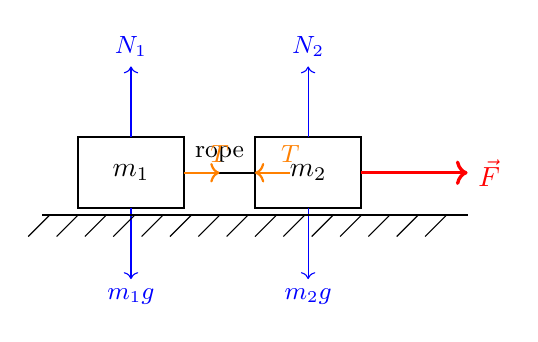
\begin{tikzpicture}[scale=0.9]
    % Two blocks
    \draw[thick] (0,0) rectangle (1.5,1) node[midway]{$m_1$};
    \draw[thick] (2.5,0) rectangle (4,1) node[midway]{$m_2$};
    % Rope
    \draw[thick] (1.5,0.5) -- (2.5,0.5) node[above,midway]{\small rope};
    % Applied force
    \draw[->,very thick,red] (4,0.5) -- (5.5,0.5) node[right]{$\vec{F}$};
    % Normal forces
    \draw[->,blue] (0.75,1) -- (0.75,2) node[above]{\small $N_1$};
    \draw[->,blue] (3.25,1) -- (3.25,2) node[above]{\small $N_2$};
    % Weights
    \draw[->,blue] (0.75,0) -- (0.75,-1) node[below]{\small $m_1 g$};
    \draw[->,blue] (3.25,0) -- (3.25,-1) node[below]{\small $m_2 g$};
    % Tension arrows on rope
    \draw[->,thick,orange] (1.5,0.5) -- (2.0,0.5) node[above]{\small $T$};
    \draw[<-,thick,orange] (2.5,0.5) -- (3.0,0.5) node[above]{\small $T$};
    % Ground
    \draw[thick] (-0.5,-0.1) -- (5.5,-0.1);
    \foreach \x in {-0.4,-0.0,0.4,0.8,...,5.4}
      \draw[thin] (\x,-0.1) -- (\x-0.3,-0.4);
  \end{tikzpicture}
  \caption{Two blocks connected by a light rope on a frictionless surface. Horizontally,
  $m_1$ is pulled only by the tension $T$, while $m_2$ is pulled forward by $F$ and backward by $T$.}
\end{figure}


\section{The Third Law}

\begin{keybox}[The Third Law]
If object 1 exerts a force $\vec{F}_{21}$ on object 2, then object 2 will exert a reaction
force $\vec{F}_{12}$ on object 1 given by
\begin{equation}
  \vec{F}_{12} = -\vec{F}_{21}.
\end{equation}
\end{keybox}

The crucial point, and the one most often misunderstood, is that these two forces act on
\textbf{different bodies}. They therefore never cancel each other.

Let us apply this to a familiar situation. You drop an apple. The Earth pulls the apple
downward with gravitational force $F=mg$. By the third law, the apple must pull the Earth
upward with an equal force. The apple's acceleration is
\begin{equation}
  a_\text{apple} = \frac{F}{m_\text{apple}} = g \approx 9.8\;\text{m/s}^2.
\end{equation}
The Earth's acceleration is
\begin{equation}
  a_\text{Earth} = \frac{F}{M_\text{Earth}} = \frac{mg}{M_\text{Earth}}.
\end{equation}
Taking a 100\,g apple and $M_\text{Earth}\approx5.97\times10^{24}\,\text{kg}$:
\begin{equation}
  a_\text{Earth} \approx 1.6\times10^{-25}\;\text{m/s}^2.
\end{equation}
Over the roughly half-second duration of the apple's fall, the Earth moves toward the apple
by a distance far smaller than the diameter of a proton.

The principle scales up. The third law is also at the root of the \textbf{horse-cart paradox}.
A horse pulls a cart forward. By the third law, the cart pulls the horse backward with an
equal force. So how does anything ever move? The resolution: the forward pull on the cart
and the backward pull on the horse act on \emph{different bodies}. To understand the horse's
motion we must look at all forces on the horse, which includes not only the backward pull
from the cart but also the forward friction from the ground on its hooves. Both the horse
and cart accelerate together. No paradox, only careful bookkeeping.


\section*{Class Exercise: The Atwood Machine}
\addcontentsline{toc}{section}{Class Exercise: The Atwood Machine}

Two blocks are connected by a light, inextensible string passing over a small frictionless
pulley fixed to the ceiling. Block 1 has mass $m_1=6\,\text{kg}$ and Block 2 has mass
$m_2=4\,\text{kg}$. The system is released from rest. Take $g=10\,\text{m/s}^2$.

\begin{figure}[H]
  \centering
  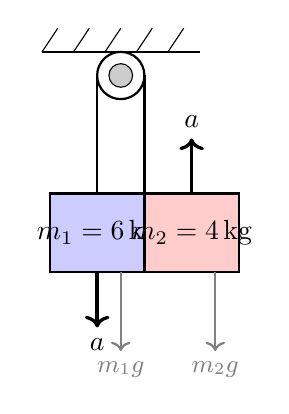
\begin{tikzpicture}
    % Pulley
    \draw[thick] (0,0) circle (0.3);
    \draw[fill=gray!40] (0,0) circle (0.15);
    % Ceiling
    \draw[thick] (-1,0.3) -- (1,0.3);
    \foreach \x in {-1,-0.6,...,0.9}
      \draw[thin] (\x,0.3) -- (\x+0.2,0.6);
    % Strings
    \draw[thick] (-0.3,0) -- (-0.3,-1.5);
    \draw[thick] (0.3,0)  -- (0.3,-1.5);
    % Blocks
    \draw[thick,fill=blue!20] (-0.9,-1.5) rectangle (0.3,-2.5) node[midway]{$m_1=6\,\text{kg}$};
    \draw[thick,fill=red!20]  (0.3,-1.5)  rectangle (1.5,-2.5) node[midway]{$m_2=4\,\text{kg}$};
    % Acceleration arrows
    \draw[->,very thick] (-0.3,-2.5) -- (-0.3,-3.2) node[below]{$a$};
    \draw[->,very thick] (0.9,-1.5) -- (0.9,-0.8) node[above]{$a$};
    % Weight labels
    \draw[->,thick,gray] (0,-2.5) -- (0,-3.5) node[below]{\small $m_1 g$};
    \draw[->,thick,gray] (1.2,-2.5) -- (1.2,-3.5) node[below]{\small $m_2 g$};
  \end{tikzpicture}
  \caption{The Atwood Machine. Block 1 ($m_1=6\,\text{kg}$) descends while Block 2 ($m_2=4\,\text{kg}$) ascends.}
\end{figure}

\begin{enumerate}[label=(\alph*)]
  \item Draw a free body diagram for each block and write down Newton's second law for each.
  \item Hence find the acceleration $a$ of the system and the tension $T$ in the string.
  \item What is the tension in the string if both masses were equal? Comment on your answer physically.
\end{enumerate}





%%-----------Chapter 5------------------------------------------
\chapter{Further Applications of Newton's Laws}

% ==============================================================
\section{Contact Forces}
% ==============================================================

Pushing, lifting and pulling are \textbf{\textit{contact forces}} that we experience in the everyday world. Rest your hand on a table; the atoms that form the molecules that make up the table and your hand are in contact with each other. If you press harder, the atoms are also pressed closer together. The electrons in the atoms begin to repel each other and your hand is pushed in the opposite direction by the table.

According to Newton's Third Law, the force of your hand on the table is equal in magnitude and opposite in direction to the force of the table on your hand. Clearly, if you push harder the force increases. If you push your hand straight down on the table, the table pushes back in a direction perpendicular (normal) to the surface. Slide your hand gently forward along the surface of the table. You barely feel the table pushing upward, but you do feel the friction acting as a resistive force to the motion of your hand. This force acts tangential to the surface and opposite to the motion of your hand. Push downward and forward. Try to estimate the magnitude of the force acting on your hand.

The force of the table acting on your hand, $\vec{F}_{c} \equiv \vec{C}$, is called the \textbf{\textit{contact force}}. This force has both a normal component to the surface, $\vec{C}_{\perp} \equiv \vec{\mathscr{N}}$, called the \textbf{\textit{normal force}}, and a tangential component to the surface, $\vec{C}_{\parallel} \equiv \vec{f}$, called the \textbf{\textit{friction force}} (Figure~\ref{fig:contactforce}).



\begin{figure}[ht]
\centering
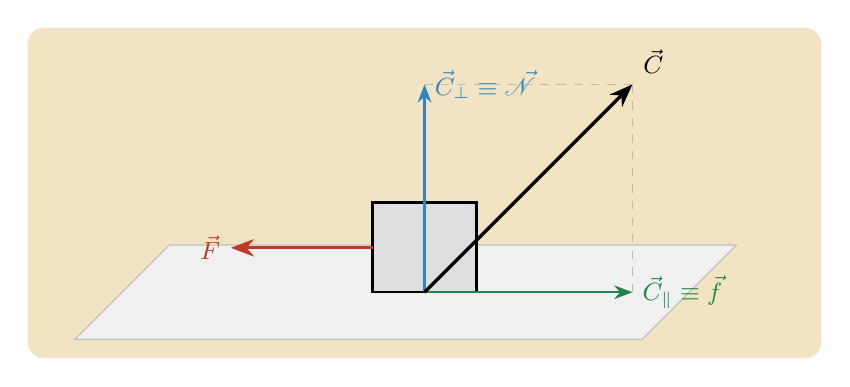
\begin{tikzpicture}[>=Stealth, thick, scale=1.2]
    % --- Warm paper background ---
    \fill[paper, rounded corners=6pt] (-3.0,-0.50) rectangle (5.4,3.0);
    
    % Surface parallelogram
    \fill[gray!12] (-2.5,-0.3) -- (3.5,-0.3) -- (4.5,0.7) -- (-1.5,0.7) -- cycle;
    \draw[gray!50, thin] (-2.5,-0.3) -- (3.5,-0.3) -- (4.5,0.7) -- (-1.5,0.7) -- cycle;
    % Block
    \fill[gray!25] (0.65, 0.2) rectangle (1.75, 1.15);
    \draw[thick] (0.65, 0.2) rectangle (1.75, 1.15);
    % Contact origin
    \coordinate (O) at (1.2, 0.2);
    % F: red, pushing left
    \draw[->, very thick, myred] (0.65, 0.67) -- ++(-1.5, 0)
        node[left, font=\small] {$\vec{F}$};
    % N: blue, up
    \draw[->, thick, myblue] (O) -- ++(0, 2.2)
        node[right, font=\small] {$\vec{C}_\perp \equiv \vec{\mathscr{N}}$};
    % f: green, horizontal right
    \draw[->, thick, mygreen] (O) -- ++(2.2, 0)
        node[right, font=\small] {$\vec{C}_{\parallel} \equiv \vec{f}$};
    % C: black, resultant
    \draw[->, very thick, black] (O) -- ++(2.2, 2.2)
        node[above right, font=\small] {$\vec{C}$};
    % Dashed construction lines
    \draw[dashed, gray!55, thin] (O) ++(0, 2.2) -- ++(2.2, 0);
    \draw[dashed, gray!55, thin] (O) ++(2.2, 0) -- ++(0, 2.2);
\end{tikzpicture}
\caption{The block is pushed to the left by $\vec{F}$. The contact force $\vec{C}$ decomposes into a normal component $\vec{\mathscr{N}}$ and a tangential friction component $\vec{f}$ opposing the motion.}
\label{fig:contactforce}
\end{figure}



The contact force, written in terms of its component forces, is therefore
\begin{equation}
    \vec{C} = \vec{C}_\perp + \vec{C}_{\parallel} \equiv \vec{\mathscr{N}} + \vec{f}\,.
\end{equation}
The normal component $\vec{\mathscr{N}}$ and the tangential component $\vec{f}$ are not independent forces but the vector components of the contact force, perpendicular and parallel to the surface of contact. 



% ==============================================================
\section*{Friction}
% ==============================================================

When a block slides along a horizontal surface or down an inclined plane, a lateral force resists the motion. Even when the block is at rest on an inclined plane, a lateral force prevents it from sliding. This resistive force is known as \textit{dry friction}, and
there are two distinguishing types when surfaces are in contact with each other.

When two surfaces move relative to one another, the friction is called \textbf{\textit{kinetic friction}} (or \textbf{\textit{sliding friction}}). When the surfaces are stationary relative to each other but a lateral force is present, the friction is called \textbf{\textit{static friction}}.

\begin{predictbox}[5.1: The brick, flat or standing?]
Take a brick (or this textbook). You can drag it lying \emph{flat} (large face
down) or standing on its \emph{edge} (small face down). The weight is the same
either way; only the contact area changes --- by a factor of three or four.
Predict: to slide it at steady speed, which orientation needs the harder
pull? Flat, on edge, or no difference? Write your answer down with a one-line
reason --- then, if a spring scale or a rubber band is handy, test it before
reading on.
\end{predictbox}

You have just repeated, with a brick, the experiments Leonardo da Vinci
recorded in his notebooks over the years 1493 to about 1515 --- the first
systematic measurements of kinetic friction ever made. Dragging blocks with
hanging weights and pulleys, he found the two facts that still carry his
fingerprints today: the force needed to slide a block is proportional to how
hard the surfaces are pressed together, and --- the surprise --- it does
\emph{not} depend on the area of contact. Da Vinci never published; his
results were rediscovered and published by Guillaume Amontons in 1699, and
extended by Charles-Augustin Coulomb, who showed that kinetic friction is
also independent of sliding speed for ordinary speeds. Hold on to your brick
prediction; the second of da Vinci's facts will grade it in a moment.

\subsection{Kinetic Friction}

The magnitude of the kinetic friction force $\vec{f}^{\,k}$ is proportional to the normal force between the two surfaces,
\begin{equation}
    f_k = \mu_k \mathscr{N}\,,
\end{equation}
where $\mu_k$ is the \textbf{\textit{coefficient of kinetic friction}}, a dimensionless constant depending only on the two materials in contact. Now look at what this law does \emph{not} contain: the contact area. The flat brick and the standing brick need exactly the same pull --- if your prediction in Stop and Predict 5.1 said otherwise, you are with the majority, and with common sense; but the experiment (da Vinci's and yours) says no difference. Two blocks of the same mass but different footprints require the same force to slide at constant speed (Figure~\ref{fig:kineticarea}). Roughly speaking: the flat brick spreads its weight over more contact points, but presses each one more lightly; the standing brick concentrates the same weight on fewer, harder-pressed points. The two effects cancel. This follows from the microscopic structure of surfaces, as discussed in the next section.

\begin{figure}[ht]
\centering
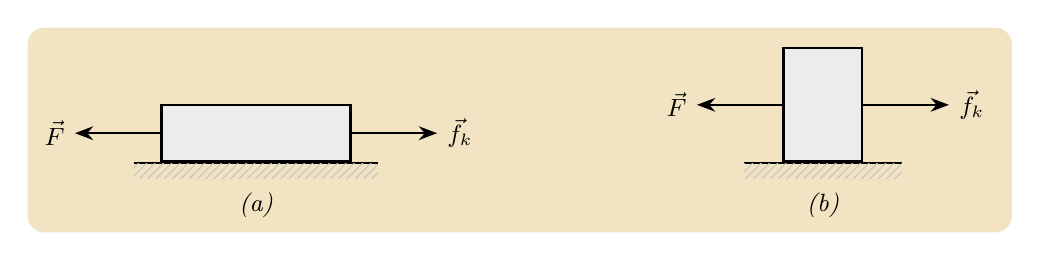
\begin{tikzpicture}[>=Stealth, thick]
    % --- Warm paper background ---
    \fill[paper, rounded corners=6pt] (-6.5,-0.9) rectangle (6,1.7);
    \begin{scope}[shift={(-3.6,0)}]
        \draw[thick] (-1.55,-0.02) -- (1.55,-0.02);
        \fill[pattern=north east lines, pattern color=gray!45]
            (-1.55,-0.22) rectangle (1.55,-0.02);
        \draw[fill=gray!15] (-1.2,0) rectangle (1.2,0.72);
        \draw[->, thick] (-1.2,0.36) -- ++(-1.1,0)
            node[left, font=\small] {$\vec{F}$};
        \draw[->, thick] ( 1.2,0.36) -- ++( 1.1,0)
            node[right, font=\small] {$\vec{f}_k$};
        \node[font=\small\itshape] at (0,-0.55) {(a)};
    \end{scope}
    \begin{scope}[shift={(3.6,0)}]
        \draw[thick] (-1.0,-0.02) -- (1.0,-0.02);
        \fill[pattern=north east lines, pattern color=gray!45]
            (-1.0,-0.22) rectangle (1.0,-0.02);
        \draw[fill=gray!15] (-0.5,0) rectangle (0.5,1.44);
        \draw[->, thick] (-0.5,0.72) -- ++(-1.1,0)
            node[left, font=\small] {$\vec{F}$};
        \draw[->, thick] ( 0.5,0.72) -- ++( 1.1,0)
            node[right, font=\small] {$\vec{f}_k$};
        \node[font=\small\itshape] at (0,-0.55) {(b)};
    \end{scope}
\end{tikzpicture}
\caption{Kinetic friction is independent of contact area. Block~(a) has twice the footprint of block~(b), yet both require the same force to slide at constant speed.}
\label{fig:kineticarea}
\end{figure}

\subsection{Static Friction}

Static friction does not take a fixed value; it adjusts itself to prevent relative motion. As you push a stationary block with increasing force, static friction matches your push exactly until a maximum value is reached. Beyond this threshold, the block slips and kinetic friction takes over. The magnitude of static friction therefore satisfies
\begin{equation}
    0 \leq f_s \leq (f_s)_{\max}\,,
\end{equation}
where the maximum is found experimentally to be proportional to the normal force,
\begin{equation}
    (f_s)_{\max} = \mu_s \mathscr{N}\,.
\end{equation}
Here $\mu_s$ is the \textbf{\textit{coefficient of static friction}}. Experiment consistently gives $\mu_s > \mu_k$: more force is needed to initiate sliding than to sustain it. This small difference accounts for the stick-slip behaviour of chalk on a blackboard, fingernails on glass, or a violin bow on a string.

The direction of static friction always opposes the applied force, as shown in Figure~\ref{fig:staticdir}.

\begin{figure}[ht]
\centering
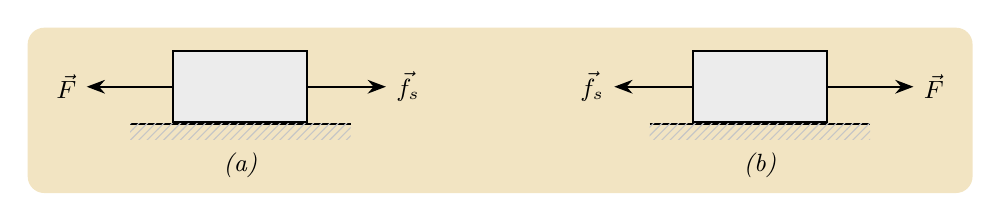
\begin{tikzpicture}[>=Stealth, thick]
    \fill[paper, rounded corners=6pt] (-6.0,-0.9) rectangle (6,1.2);
    \begin{scope}[shift={(-3.3,0)}]
        \draw[thick] (-1.4,-0.02) -- (1.4,-0.02);
        \fill[pattern=north east lines, pattern color=gray!45]
            (-1.4,-0.22) rectangle (1.4,-0.02);
        \draw[fill=gray!15] (-0.85,0) rectangle (0.85,0.9);
        \draw[->, thick] (-0.85,0.45) -- ++(-1.1,0)
            node[left,  font=\small] {$\vec{F}$};
        \draw[->, thick] ( 0.85,0.45) -- ++( 1.0,0)
            node[right, font=\small] {$\vec{f}_s$};
        \node[font=\small\itshape] at (0,-0.55) {(a)};
    \end{scope}
    \begin{scope}[shift={(3.3,0)}]
        \draw[thick] (-1.4,-0.02) -- (1.4,-0.02);
        \fill[pattern=north east lines, pattern color=gray!45]
            (-1.4,-0.22) rectangle (1.4,-0.02);
        \draw[fill=gray!15] (-0.85,0) rectangle (0.85,0.9);
        \draw[->, thick] ( 0.85,0.45) -- ++( 1.1,0)
            node[right, font=\small] {$\vec{F}$};
        \draw[->, thick] (-0.85,0.45) -- ++(-1.0,0)
            node[left,  font=\small] {$\vec{f}_s$};
        \node[font=\small\itshape] at (0,-0.55) {(b)};
    \end{scope}
\end{tikzpicture}
\caption{Static friction opposes the applied force. In~(a) $\vec{F}$ acts to the left so $\vec{f}_s$ acts to the right. In~(b) the roles are reversed.}
\label{fig:staticdir}
\end{figure}

Two important distinctions between static and kinetic friction are worth keeping in mind.
\vspace{-0.1cm}
\begin{enumerate}[leftmargin=2em, itemsep=2pt]
    \item The magnitude and direction of static friction depend on the applied forces and adjust to maintain equilibrium, up to the maximum $(f_s)_{\max}$. Kinetic friction, by contrast, has a fixed magnitude $\mu_k \mathscr{N}$ for a given normal force.
    \item When the applied force along the contact surface reaches $(f_s)_{\max}$, the surfaces begin to slip. This threshold condition is called the \textbf{\textit{just slipping}} condition, and marks the transition from static to kinetic friction.
\end{enumerate}

\vspace{0.3cm}

\begin{workedexample}[5.1: Sliding Block]
A block of mass \(m\) slides down an incline of angle \(30^\circ\) with an acceleration \(g/4\). Find the kinetic friction coeffcient \(\mu_k\).


\medskip
\textit{Solution.}
We resolve the forces into components parallel and perpendicular to the incline, taking
the positive direction down the slope for motion and outward from the surface for the
normal direction. 

\begin{center}
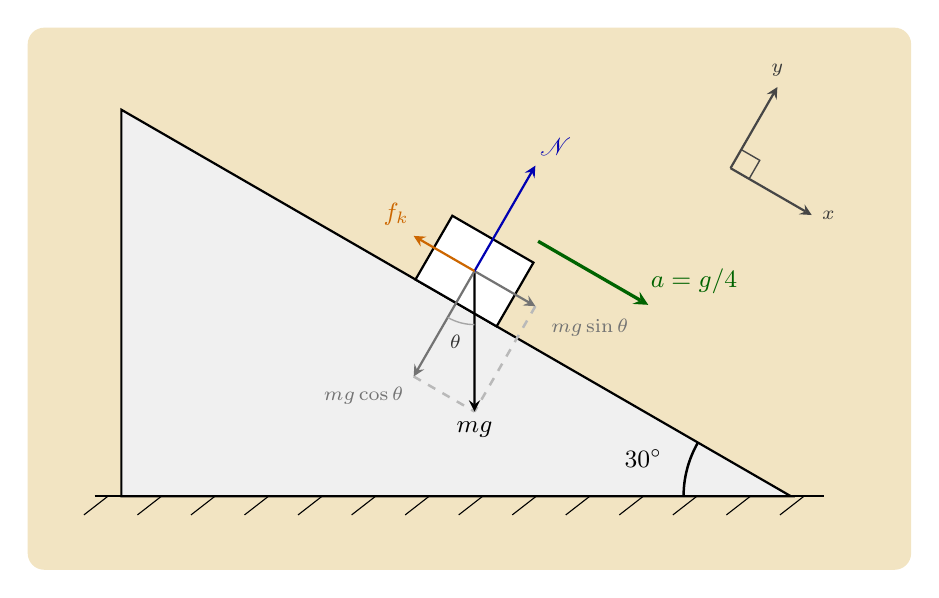
\begin{tikzpicture}[scale=1.7, line width=0.9pt, >=stealth]

    \pgfmathsetmacro{\ang}{30}

    % --- Warm paper background ---
    \fill[paper, rounded corners=6pt] (-0.7,-0.55) rectangle (5.9,3.5);

    % --- Incline triangle ---
    \coordinate (A) at (0,0);
    \coordinate (B) at (5,0);
    \coordinate (C) at (0, {5*tan(\ang)});
    \draw[thick, fill=gray!12] (A) -- (B) -- (C) -- cycle;

    % Ground hatch
    \draw[thick] (-0.2,0) -- (5.25,0);
    \foreach \x in {-0.1,0.3,0.7,1.1,1.5,1.9,2.3,2.7,3.1,3.5,3.9,4.3,4.7,5.1}
        \draw[thin] (\x,0) -- +(-0.18,-0.14);

    % Angle at B
    \draw (4.2,0) arc (180:{180-\ang}:0.8);
    \node at (3.9,0.28) {\small $30^\circ$};

    % --- Block position on slope ---
    \pgfmathsetmacro{\bx}{5 - 0.50*5}
    \pgfmathsetmacro{\by}{0.50*5*tan(\ang)}
    \pgfmathsetmacro{\bcx}{\bx + 0.275*cos(60)}
    \pgfmathsetmacro{\bcy}{\by + 0.275*sin(60)}
    \coordinate (O) at (\bcx,\bcy);

    \begin{scope}[shift={(O)}, rotate={-\ang}]
        \draw[fill=white, thick] (-0.35,-0.275) rectangle (0.35,0.275);
    \end{scope}

    % --- Lengths (shortened) ---
    \pgfmathsetmacro{\L}{1.05}
    \pgfmathsetmacro{\Lsin}{\L*sin(\ang)}
    \pgfmathsetmacro{\Lcos}{\L*cos(\ang)}

    \coordinate (mgTip)   at ($(O)+(270:\L)$);
    \coordinate (sinTip)  at ($(O)+(-\ang:\Lsin)$);
    \coordinate (cosTip)  at ($(O)+(240:\Lcos)$);

    % --- Dashed parallelogram of components ---
    \draw[dashed, gray!55] (sinTip) -- (mgTip);
    \draw[dashed, gray!55] (cosTip) -- (mgTip);

    % --- Weight and components ---
    \draw[->, thick, black] (O) -- (mgTip)
        node[below, font=\small] {$mg$};
    \draw[->, thick, black!55] (O) -- (sinTip)
        node[below right, font=\scriptsize, xshift=2pt, yshift=-1pt] {$mg\sin\theta$};
    \draw[->, thick, black!55] (O) -- (cosTip)
        node[below left, font=\scriptsize] {$mg\cos\theta$};

    % --- angle theta between mg and mg cos th ---
    \draw[line width=0.5pt, gray!70] (O)+(270:0.40) arc (270:240:0.40);
    \node[font=\scriptsize, gray!40!black] at ($(O)+(255:0.55)$) {$\theta$};

    % --- Normal force ---
    \draw[->, thick, blue!70!black] (O) -- ($(O)+(60:\Lcos)$)
        node[above right, font=\small, xshift=-2pt] {$\mathscr{N}$};

    % --- Friction ---
    \draw[->, thick, orange!80!black] (O) -- ($(O)+(150:\Lsin)$)
        node[above left, font=\small, xshift=2pt] {$f_k$};

    % --- Acceleration g/4 ---
    \coordinate (aStart) at ($(O)+(60:0.43)+(-30:0.30)$);
    \draw[->, very thick, green!39!black] (aStart) -- ++(-\ang:0.95)
        node[above right, font=\small, xshift=-3pt] {$a=g/4$};

    % --- Coordinate axes inset ---
    \coordinate (Oax) at (4.55,2.45);
    \draw[->, gray!55!black, line width=0.8pt]
        (Oax) -- ($(Oax)+(-\ang:0.7)$) node[right, font=\scriptsize, gray!45!black] {$x$};
    \draw[->, gray!55!black, line width=0.8pt]
        (Oax) -- ($(Oax)+(60:0.7)$) node[above, font=\scriptsize, gray!45!black] {$y$};
    \draw[gray!55!black, line width=0.5pt]
        ($(Oax)+(-\ang:0.16)$) -- ($(Oax)+(-\ang:0.16)+(60:0.16)$) -- ($(Oax)+(60:0.16)$);

\end{tikzpicture}
\end{center}


\vspace{0.3cm}
Perpendicular to the incline there is no acceleration, so the normal force balances the
perpendicular component of gravity,
\begin{equation*}
    \mathscr{N} - mg\cos\theta = 0 \implies \mathscr{N} = mg\cos\theta.
\end{equation*}

Along the incline, the block accelerates down the slope at $a = g/4$. The driving force is
the parallel component of gravity, $mg\sin\theta$, opposed by kinetic friction
$f_k = \mu_k\mathscr{N}$ acting up the slope. Newton's second law gives
\begin{equation*}
    mg\sin\theta - \mu_k\mathscr{N} = ma.
\end{equation*}
Substituting $\mathscr{N} = mg\cos\theta$ and $a = g/4$,
\begin{equation*}
    mg\sin\theta - \mu_k mg\cos\theta = \tfrac{1}{4}mg.
\end{equation*}
The mass $m$ and the acceleration $g$ cancel throughout, leaving a relation among pure
numbers,
\begin{equation*}
    \sin\theta - \mu_k\cos\theta = \tfrac{1}{4}.
\end{equation*}
Solving for the coefficient of kinetic friction,
\begin{equation*}
    \mu_k = \frac{\sin\theta - \tfrac{1}{4}}{\cos\theta}.
\end{equation*}
With $\theta = 30^\circ$, so that $\sin\theta = \tfrac{1}{2}$ and $\cos\theta = \tfrac{\sqrt{3}}{2}$,
\begin{equation*}
    \mu_k = \frac{1/2 - 1/4}{\sqrt{3}/2}
          = \frac{1}{2\sqrt{3}}.
\end{equation*}



\end{workedexample}


\newpage


\section*{The Normal Force}

When two solid bodies are pressed together, their surfaces resist interpenetration.
Push your hand against a wall and the wall pushes back, preventing your hand from
passing through (Figure~\ref{fig:stickwall}). This perpendicular push is called the
\textit{normal force}, where \textit{normal} means perpendicular to the surface of
contact. Notice that the harder you push on the wall with a force $\vec{F}$, the harder
the wall pushes back on your hand with the normal force $\vec{\mathscr{N}}$.

The origin of this force is atomic. The atoms at the surface of your hand and the
atoms at the surface of the wall repel one another the moment they come into contact,
opposing any further compression. The material of the wall behaves, at the microscopic
level, like an array of tiny springs.\footnote{The ``atomic springs'' picture is a
useful analogy but not the complete story. The true origin of this repulsion is quantum
mechanical: as electron clouds overlap, the Pauli exclusion principle forces electrons
into higher energy states, giving rise to a repulsive force. Classical electrostatics
plays a secondary role. We will encounter the Pauli exclusion principle when we study
modern physics.} When you push against the wall, these atomic springs compress
slightly, and the repulsive force they exert grows with the compression until it exactly
balances your push. For a hard material such as concrete, the compression is so small
as to be invisible, and the wall appears perfectly rigid.

This is why the normal force is not a fixed quantity: it adjusts itself to match whatever
force is pressing the surfaces together. Push harder, and the atomic springs compress
more, increasing the normal force in response. As the figure shows, $\vec{F}$ and
$\vec{\mathscr{N}}$ always grow together and remain equal in magnitude. The normal force is
therefore a \textit{constraint force}, one whose magnitude is determined not by a fixed
law but by the condition that the two surfaces do not pass through each other.


\begin{figure}[ht!]
\centering
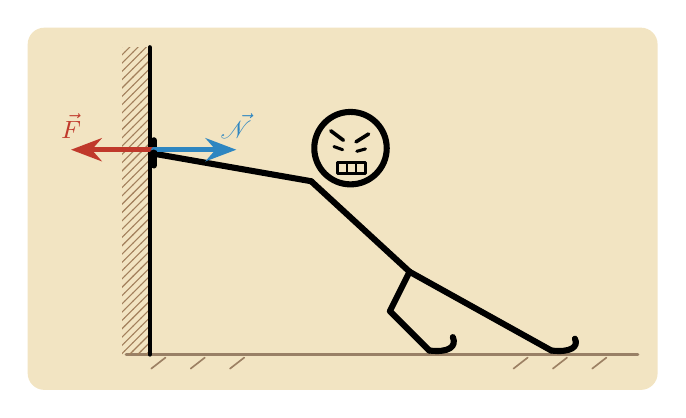
\begin{tikzpicture}[scale=1.0, line cap=round, line join=round, >=Stealth]

    \tikzset{limb/.style={line width=2.2pt, black}}

    % --- Warm paper background ---
    \fill[paper, rounded corners=6pt] (-1.55,-0.45) rectangle (6.45,4.15);

    % --- Ground ---
    \draw[line width=1pt, gray!60!brown] (-0.3,0) -- (6.2,0);
    \foreach \x in {0.2,0.7,1.2,4.8,5.3,5.8} {
        \draw[gray!55!brown, line width=0.6pt] (\x,-0.04) -- (\x-0.18,-0.18);
    }

    % --- Wall ---
    \fill[pattern=north east lines, pattern color=gray!45!brown]
        (-0.35,0) rectangle (0,3.9);
    \draw[line width=1.6pt] (0,0) -- (0,3.9);

    % ===== Stick figure =====
    \coordinate (hand)     at (0.05, 2.55);
    \coordinate (shoulder) at (2.05, 2.20);
    \coordinate (hip)      at (3.30, 1.05);
    \coordinate (kneeF)    at (3.05, 0.55);
    \coordinate (footF)    at (3.55, 0.05);
    \coordinate (footB)    at (5.10, 0.05);

    \draw[limb] (hand) -- (shoulder);
    \draw[limb] (0.05,2.40) -- (0.05,2.72);
    \draw[limb] (shoulder) -- (hip);
    \draw[limb] (hip) -- (footB);
    \draw[limb] (footB) .. controls (5.35,0.02) and (5.45,0.10) .. (5.40,0.20);
    \draw[limb] (hip) -- (kneeF) -- (footF);
    \draw[limb] (footF) .. controls (3.80,0.02) and (3.90,0.10) .. (3.85,0.22);

    % --- Head with strained expression ---
    \draw[limb, fill=paper] (2.55,2.62) circle (0.46);
    \draw[line width=1.3pt] (2.30,2.84) -- (2.46,2.72);
    \draw[line width=1.3pt] (2.78,2.80) -- (2.62,2.70);
    \draw[line width=1.1pt] (2.34,2.64) -- (2.45,2.60);
    \draw[line width=1.1pt] (2.74,2.61) -- (2.63,2.58);
    \draw[line width=1.1pt, fill=paper] (2.38,2.30) rectangle (2.74,2.44);
    \draw[line width=0.7pt] (2.50,2.30) -- (2.50,2.44);
    \draw[line width=0.7pt] (2.62,2.30) -- (2.62,2.44);

    % --- Force arrows, both anchored at the hand ---
    \draw[->, line width=1.8pt, myred]
        (0.05,2.6) -- ++(-1.05,0) node[above, font=\small] {$\vec{F}$};
    \draw[->, line width=1.8pt, myblue]
        (0.05,2.6) -- ++(1.05,0) node[above, font=\small] {$\vec{\mathscr{N}}$};
    \fill[black] (hand) circle (1.5pt);

\end{tikzpicture}
\caption{When you push against a wall ($\vec{F}$), the wall pushes back on your hand
with an equal and opposite normal force ($\vec{\mathscr{N}}$), perpendicular to its surface.
Both forces act at the point of contact.}
\label{fig:stickwall}
\end{figure}



\section*{The Normal Force and Weight}

We say we are measuring our weight when we step onto a bathroom scale. But what is the scale actually measuring?

Two forces act on a person standing on a scale (Figure~\ref{fig:scale}). The first is the gravitational force $\vec{F}_g = m\vec{g}$, directed downward. The second is the contact force from the scale; because the person is at rest, this contact force is purely normal and we write it as $\vec{\mathscr{N}}$, directed upward. Since the person is at rest, the vertical acceleration is zero, and Newton's Second Law gives
\begin{equation}
    \vec{\mathscr{N}} + \vec{F}_g = \vec{0}.
\end{equation}
Taking the positive direction upward, this becomes
\begin{equation}
    \mathscr{N} - mg = 0 \implies \mathscr{N} = mg.
\end{equation}

It is worth being precise about four quantities that are easy to confuse. The \textit{true mass} $m$ is the amount of matter in the person, an invariant property that does not change with motion or location.\footnote{Newtonian mechanics treats mass as a fixed quantity. Special relativity shows that an object's inertia grows with its speed. One common way to express this
introduces a velocity-dependent mass $m = m_0/\sqrt{1 - v^2/c^2}$, where $m_0$ is the
rest mass and $c$ is the speed of light; for everyday speeds $v \ll c$ this is
indistinguishable from $m_0$. Modern physics usually prefers instead to keep mass as
the invariant $m_0$ and describe the growing inertia through momentum and energy. Either
way, the effect is utterly negligible at ordinary speeds. We will return to this when we
study modern physics.} The \textit{true weight} $mg$ is the actual gravitational force the Earth exerts on the person. The scale, however, does not measure either of these directly. It measures the normal force $\mathscr{N}$ pressing on it, which we call the \textit{apparent weight}. Dividing by $g$, it displays a number in kilograms, the \textit{apparent mass} $\mathscr{N}/g$. At rest the apparent mass equals the true mass and the distinction seems academic. The elevator, discussed in the next section, will reveal the difference.

The word ``weight'' is often used loosely to mean the gravitational force the Earth exerts on an object. We shall always call that force the \textit{gravitational force} rather than ``weight'', to keep it distinct from what a scale reads. When you jump into the air you feel ``weightless'' because no normal force acts on you, even though the Earth still pulls you down. You have not turned gravity off.

A common misconception deserves to be addressed before we proceed. The normal force and the gravitational force are two completely different forces. They are equal in magnitude here only because the person is at rest, and this equality will fail the moment there is acceleration. More importantly, they do not form a Newton's Third Law interaction pair: both act on the same object (the person), whereas Third Law pairs always act on \textit{different} objects. The true Third Law partner of the gravitational force on the person due to the Earth, $\vec{F}^{\,g}_{E,P}$, is the gravitational force on the Earth due to the person,  $\vec{F}^{\,g}_{P,E}$, and they satisfy \(\vec{F}^{\,g}_{E,P} = -\vec{F}^{\,g}_{P,E}\). These act on different objects: one on the person, the other on the Earth. Likewise, the Third Law partner of the normal force $\vec{\mathscr{N}}$ from the scale is the force the person's feet exert downward on the scale surface.


\section*{Experience in an Elevator}

Now we take the bathroom scale somewhere interesting. If a scale measures
the normal force --- not gravity --- then the reading should change whenever the
normal force has to do something other than just hold you up. An elevator is
the perfect laboratory: it can accelerate up, accelerate down, cruise, and
(in a thought experiment we will keep hypothetical) drop freely.

\begin{predictbox}[5.2: Four rides on a scale]
A 60\,kg person stands on a scale in an elevator. At rest the scale reads
60.0\,kg. Predict --- more than 60, less than 60, exactly 60, or zero? --- for
each ride, \emph{before} reading the analysis:
\begin{enumerate}[leftmargin=2em, itemsep=1pt]
  \item The elevator moves \emph{upward at a steady} $5\,\mathrm{m/s}$.
  \item The elevator \emph{accelerates upward}.
  \item The elevator \emph{accelerates downward} (slowing while going up, or
        speeding up while going down).
  \item The cable snaps and the elevator \emph{falls freely}.
\end{enumerate}
Ride 1 is the one people argue about longest --- ``moving up'' feels like it
should read more. Commit to all four; the next pages check them one by one.
\end{predictbox}

\noindent\textit{On the companion site:} the \textbf{elevator simulator}
(\texttt{Chapter 5} on the course website) has an acceleration slider and a
live scale readout --- test your four predictions there before or after the
analysis, and watch the cable snap in case~4.

In each case exactly two forces act on the person: the gravitational force $m\vec{g}$
directed downward and the normal force $\vec{\mathscr{N}}$ directed upward.
 
\vspace{0.3cm}
\noindent\textbf{\sffamily(a)\; At Rest or Moving at Constant Velocity.}
 
\begin{minipage}[t]{0.55\textwidth}
\vspace{0pt}
When the elevator is stationary or moving at constant velocity, the acceleration is zero.
The person's state of motion is not changing, so the floor need only support the person's
weight, nothing more. Newton's second law in the vertical direction gives
\begin{equation*}
    \vec{\mathscr{N}} + \vec{F}_g = \vec{0}
    \implies \mathscr{N} - mg = 0,
\end{equation*}
so that
\begin{equation*}
    \mathscr{N} = mg = (60)(10) = 600\;\mathrm{N}.
\end{equation*}
The scale displays $\mathscr{N}/g = 60.0\,\mathrm{kg}$. Here the apparent weight equals the
true weight, which is why we never notice the distinction in ordinary standing.
Note what this settles about ride~1 of your predictions: a steady
$5\,\mathrm{m/s}$ upward is \emph{zero acceleration}, so the scale reads
exactly 60.0 --- the reading cares about acceleration, never about velocity.
If a sealed elevator cruises perfectly smoothly, no scale (and no sensation
in your stomach) can tell you whether you are moving at all. That is the
first law speaking.
\end{minipage}
\hfill
\begin{minipage}[t]{0.6\textwidth}
\vspace{0pt}
\centering
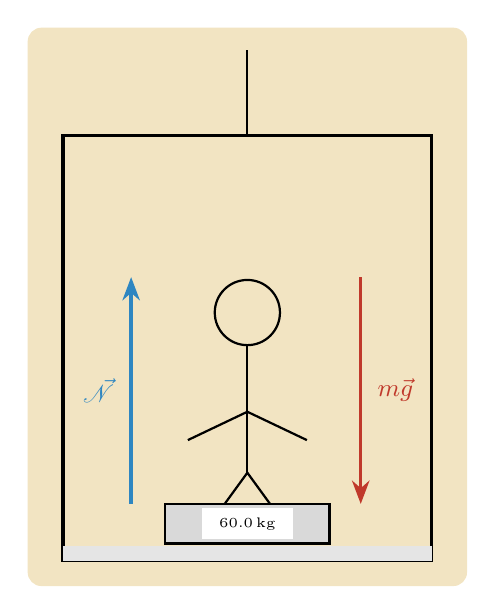
\begin{tikzpicture}[>=Stealth, scale=1.80]
    \fill[paper, rounded corners=5pt] (-1.55,-0.18) rectangle (1.55,3.76);
    \draw[very thick] (-1.3,0) rectangle (1.3,3.0);
    \draw[thick] (0,3.6) -- (0,3.0);
    \fill[gray!20] (-1.3,0) rectangle (1.3,0.10);
    \fill[gray!30] (-0.58,0.12) rectangle (0.58,0.40);
    \draw[thick]   (-0.58,0.12) rectangle (0.58,0.40);
    \fill[white]   (-0.32,0.15) rectangle (0.32,0.37);
    \node[font=\tiny] at (0,0.26) {60.0\,kg};
    \draw[thick] (-0.16,0.40) -- (0,0.62) -- (0.16,0.40);
    \draw[thick] (0,0.62) -- (0,1.52);
    \draw[thick] (0,1.05) -- (-0.42,0.85);
    \draw[thick] (0,1.05) -- ( 0.42,0.85);
    \draw[thick,fill=paper] (0,1.75) circle (0.23);
    \draw[very thick,-Stealth,myblue]  (-0.82,0.40) -- (-0.82,2.0);
    \node[left,myblue,font=\small] at (-0.87,1.20) {$\vec{\mathscr{N}}$};
    \draw[very thick,-Stealth,myred]   ( 0.80,2.00) -- ( 0.80,0.40);
    \node[right,myred,font=\small] at (0.85,1.20) {$m\vec{g}$};
\end{tikzpicture}
\label{fig:scale}
\end{minipage}

 
\vspace{2.4cm}
\noindent\textbf{\sffamily(b)\; Accelerating Upward.}
 
\noindent
\begin{minipage}[t]{0.55\textwidth}
\vspace{0pt}
Now the elevator accelerates upward. To make the person accelerate upward too, there must
be a net upward force on them. But the person's inertia resists this change in motion: their
body ``wants'' to stay at rest or moving as it was. The floor must therefore push up harder than before, hard enough both to support the weight and to supply the extra upward force the acceleration
demands. The normal force rises above $mg$. Newton's second law gives
\begin{equation}
    \mathscr{N} - mg = ma \implies \mathscr{N} = m(g+a).
\end{equation}
Suppose the scale reads $64.8\,\mathrm{kg}$, meaning $\mathscr{N} = 648\,\mathrm{N}$:
\begin{equation*}
    648 = 60(10+a) \implies a = 0.8\;\mathrm{m\,s^{-2}}\;\text{upward.}
\end{equation*}
The person feels heavier because the floor genuinely presses harder on their feet. The true
weight is unchanged at $600\,\mathrm{N}$; only the apparent weight has risen, to
$648\,\mathrm{N}$.

\end{minipage}%
\hfill
\begin{minipage}[t]{0.6\textwidth}
\vspace{0pt}
\centering
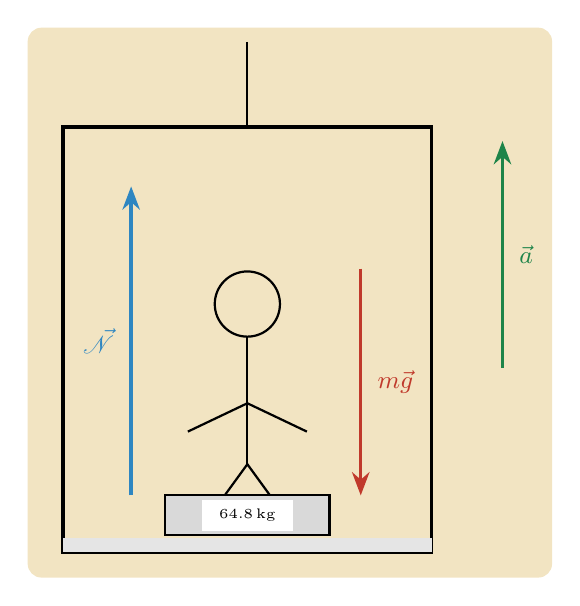
\begin{tikzpicture}[>=Stealth, scale=1.80]
    \fill[paper, rounded corners=5pt] (-1.55,-0.18) rectangle (2.15,3.7);
    \draw[very thick] (-1.3,0) rectangle (1.3,3.0);
    \draw[thick] (0,3.6) -- (0,3.0);
    \fill[gray!20] (-1.3,0) rectangle (1.3,0.10);
    \fill[gray!30] (-0.58,0.12) rectangle (0.58,0.40);
    \draw[thick]   (-0.58,0.12) rectangle (0.58,0.40);
    \fill[white]   (-0.32,0.15) rectangle (0.32,0.37);
    \node[font=\tiny] at (0,0.26) {64.8\,kg};
    \draw[thick] (-0.16,0.40) -- (0,0.62) -- (0.16,0.40);
    \draw[thick] (0,0.62) -- (0,1.52);
    \draw[thick] (0,1.05) -- (-0.42,0.85);
    \draw[thick] (0,1.05) -- ( 0.42,0.85);
    \draw[thick,fill=paper] (0,1.75) circle (0.23);
    \draw[very thick,-Stealth,myblue]  (-0.82,0.40) -- (-0.82,2.58);
    \node[left,myblue,font=\small] at (-0.87,1.49) {$\vec{\mathscr{N}}$};
    \draw[very thick,-Stealth,myred]   ( 0.80,2.00) -- ( 0.80,0.40);
    \node[right,myred,font=\small] at (0.85,1.20) {$m\vec{g}$};
    \draw[very thick,-Stealth,mygreen] (1.80,1.30) -- (1.80,2.90);
    \node[right,mygreen,font=\small] at (1.85,2.10) {$\vec{a}$};
\end{tikzpicture}
\end{minipage}



\vspace{0.3cm}
\noindent\textbf{\sffamily(c)\; Accelerating Downward.}
 
\noindent
\begin{minipage}[t]{0.55\textwidth}
\vspace{0pt}
When the elevator accelerates downward, the person's inertia resists the change: the body
"wants" to keep moving as it was, so for a moment it does not fall away with the floor as
readily as the floor drops beneath it. The person presses less firmly on the scale, and so
the scale presses less firmly back. The normal force falls below $mg$, leaving a net
downward force that produces the downward acceleration:
\begin{equation}
    mg - \mathscr{N} = ma \implies \mathscr{N} = m(g-a). \label{downward}
\end{equation}
If the scale reads $54.0\,\mathrm{kg}$, meaning $\mathscr{N} = 540\,\mathrm{N}$:
\begin{equation*}
    540 = 60(10-a) \implies a = 1.0\;\mathrm{m\,s^{-2}}\;\text{downward.}
\end{equation*}
The person feels lighter because the floor really does press less on their feet. The true
weight is unchanged at $600\,\mathrm{N}$; only the apparent weight has fallen, to
$540\,\mathrm{N}$.
\end{minipage}%
\hfill
\begin{minipage}[t]{0.60\textwidth}
\vspace{0pt}
\centering
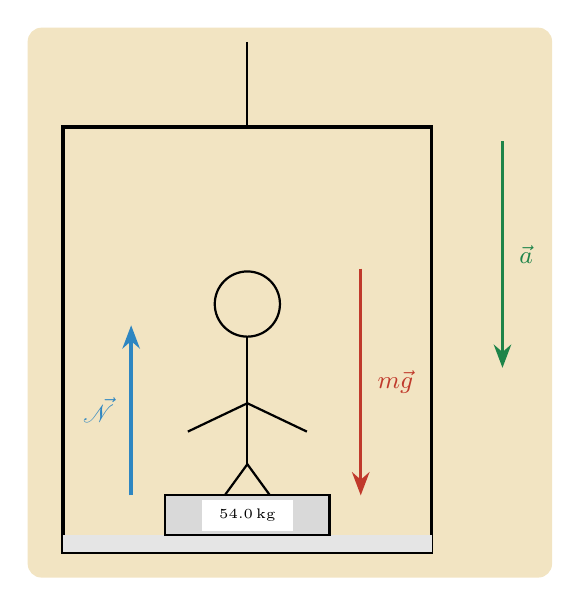
\begin{tikzpicture}[>=Stealth, scale=1.8]
    \fill[paper, rounded corners=5pt] (-1.55,-0.18) rectangle (2.15,3.7);
    \draw[very thick] (-1.3,0) rectangle (1.3,3.0);
    \draw[thick] (0,3.6) -- (0,3.0);
    \fill[gray!20] (-1.3,0) rectangle (1.3,0.12);
    \fill[gray!30] (-0.58,0.12) rectangle (0.58,0.40);
    \draw[thick]   (-0.58,0.12) rectangle (0.58,0.40);
    \fill[white]   (-0.32,0.15) rectangle (0.32,0.37);
    \node[font=\tiny] at (0,0.26) {54.0\,kg};
    \draw[thick] (-0.16,0.40) -- (0,0.62) -- (0.16,0.40);
    \draw[thick] (0,0.62) -- (0,1.52);
    \draw[thick] (0,1.05) -- (-0.42,0.85);
    \draw[thick] (0,1.05) -- ( 0.42,0.85);
    \draw[thick,fill=paper] (0,1.75) circle (0.23);
    \draw[very thick,-Stealth,myblue]  (-0.82,0.40) -- (-0.82,1.60);
    \node[left,myblue,font=\small] at (-0.87,1.00) {$\vec{\mathscr{N}}$};
    \draw[very thick,-Stealth,myred]   ( 0.80,2.00) -- ( 0.80,0.40);
    \node[right,myred,font=\small] at (0.85,1.20) {$m\vec{g}$};
    \draw[very thick,-Stealth,mygreen] (1.80,2.90) -- (1.80,1.30);
    \node[right,mygreen,font=\small] at (1.85,2.10) {$\vec{a}$};
\end{tikzpicture}
\end{minipage}
 
\vspace{1.2cm}
\noindent\textbf{\sffamily(d)\; Free Fall.}
 
\noindent
\begin{minipage}[t]{0.55\textwidth}
\vspace{0pt}
Now imagine the cable snaps and the elevator falls freely. Gravity acts on everything
inside equally, so the person, the scale, and the floor all accelerate downward together
at the same rate $a = g$. Because the floor falls away just as fast as the person does, it
never has to push on them at all. The normal force drops all the way to zero. Setting
$a = g$ in equation~\eqref{downward},
\begin{equation*}
    \mathscr{N} = m(g - g) = 0.
\end{equation*}
The scale reads zero, yet gravity has certainly not switched off; the Earth still pulls the
person down with the full force $mg$. The person simply floats inside the falling car
because there is no longer any contact force to register. This is exactly what we mean by
\textit{weightlessness}: not the absence of gravity, but the absence of the normal force.
\end{minipage}%
\hfill
\begin{minipage}[t]{0.60\textwidth}
\vspace{0pt}
\centering
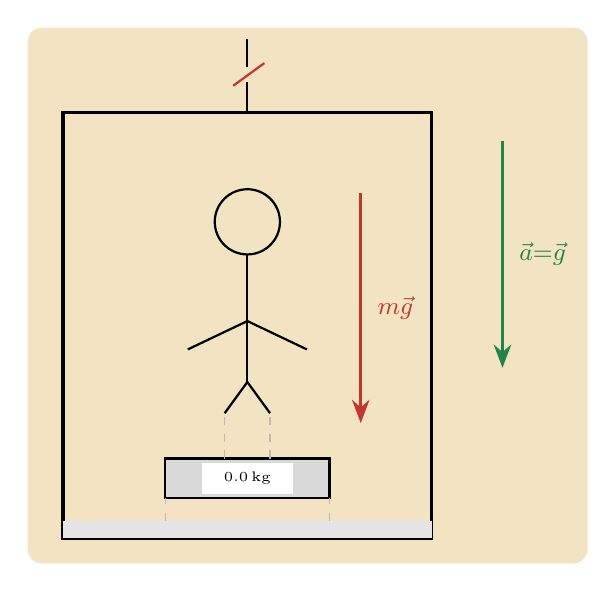
\begin{tikzpicture}[>=Stealth, scale=1.80]
    \fill[paper, rounded corners=5pt] (-1.55,0.22) rectangle (2.4,4.0);
    \draw[very thick] (-1.3,0.4) rectangle (1.3,3.4);
    \draw[thick] (0,3.4) -- (0,3.62);
    \draw[thick] (0,3.72) -- (0,3.92);
    \draw[thick, myred] (-0.10, 3.59) -- (0.12, 3.75);
    \fill[gray!20] (-1.3,0.4) rectangle (1.3,0.52);
    \fill[gray!30] (-0.58,0.68) rectangle (0.58,0.96);
    \draw[thick]   (-0.58,0.68) rectangle (0.58,0.96);
    \fill[white]   (-0.32,0.71) rectangle (0.32,0.93);
    \node[font=\tiny] at (0,0.82) {0.0\,kg};
    \draw[dashed,gray!55,thin] (-0.58,0.52) -- (-0.58,0.68);
    \draw[dashed,gray!55,thin] ( 0.58,0.52) -- ( 0.58,0.68);
    \draw[thick] (-0.16,1.28) -- (0,1.50) -- (0.16,1.28);
    \draw[thick] (0,1.50) -- (0,2.40);
    \draw[thick] (0,1.93) -- (-0.42,1.73);
    \draw[thick] (0,1.93) -- ( 0.42,1.73);
    \draw[thick,fill=paper] (0,2.63) circle (0.23);
    \draw[dashed,gray!55,thin] (-0.16,0.96) -- (-0.16,1.28);
    \draw[dashed,gray!55,thin] ( 0.16,0.96) -- ( 0.16,1.28);
    \draw[very thick,-Stealth,myred] (0.80,2.83) -- (0.80,1.21);
    \node[right,myred,font=\small] at (0.85,2.02) {$m\vec{g}$};
    \draw[very thick,-Stealth,mygreen] (1.80,3.20) -- (1.80,1.60);
    \node[right,mygreen,font=\small] at (1.85,2.40) {$\vec{a}{=}\vec{g}$};
\end{tikzpicture}
\end{minipage}
 


\begin{checkpoint}[5.1: The floating astronaut]
Astronauts on the International Space Station float freely inside the cabin.
The station orbits about 400\,km above the Earth's surface. The astronauts
float because
\begin{enumerate}[label=(\alph*), leftmargin=2.5em, itemsep=0pt]
  \item at that altitude they are beyond the reach of the Earth's gravity.
  \item the Earth's gravity is cancelled by the pull of the Moon and Sun.
  \item they and the station are both in free fall, falling around the Earth together.
  \item the station's speed generates an outward force that balances gravity.
\end{enumerate}
\checkanswer{Answer: (c). At 400 km up, the Earth's gravity is still about
90\% of its surface strength --- answer (a) is the single most common
misconception in this course. The station and everyone in it are permanently
in case (d) of the elevator: falling freely, together, all the time. Their
sideways speed simply makes them keep missing the Earth --- which is what an
orbit is, as the section on gravitation will make precise.}
\end{checkpoint}

\begin{supplementary}{A Glimpse of Something Deeper: The Equivalence Principle}

We close the elevator story with a question that troubled Einstein and ultimately led him to general relativity.
Imagine you wake up inside a sealed box with no windows. You feel a normal force pressing
up on your feet. How could you tell whether you are sitting stationary on the surface of the
Earth, with gravity pulling you down, or drifting in empty space far from any planet, with
the box accelerating upward at $g=9.8\,\text{m/s}^2$?

The remarkable answer is that you cannot. No mechanical experiment conducted inside the
box will distinguish between these two situations. Drop a ball: in both cases it accelerates
toward the floor at $10\,\text{m/s}^2$. Step on a scale: it reads $mg$ in both cases. Einstein
elevated this to a fundamental principle: \textbf{gravity and accelerated motion are locally
equivalent}. This is the \textbf{equivalence principle}.

\textbf{a) Two Kinds of Mass.} The symbol $m$ appears in two logically distinct roles.
In Newton's second law, $m$ appears as \textbf{inertial mass}: the resistance of an object to
acceleration. In the gravitational force law, $m$ appears as \textbf{gravitational mass}: the
quantity that determines how strongly gravity pulls on the object. There is no obvious reason
these two quantities should be equal. Yet every experiment ever performed finds them equal.
The Hungarian physicist Lor\'and E\"otv\"os demonstrated this equality to one part in $10^8$
in the 1880s, and modern experiments push this to one part in $10^{15}$.

The equality $m_\text{inertial}=m_\text{gravitational}$ is exactly what ensures that all
objects fall at the same rate regardless of their mass.

\textbf{b) Light Must Bend.} The equivalence principle has a striking consequence that
goes beyond mechanics. Shine a horizontal beam of light across the accelerating box. While
the light travels across, the box accelerates upward, so the beam hits the far wall slightly
below where it was aimed --- the light beam appears to curve downward. Since an accelerating
box is locally indistinguishable from a gravitational field, gravity must also bend light. This
was a radical prediction: Newtonian gravity acts only on objects with mass, and light was
thought to be massless. Einstein's prediction was confirmed experimentally in 1919 by Arthur
Eddington, who photographed stars near the edge of the Sun during a solar eclipse and found
that their apparent positions were shifted by exactly the amount Einstein predicted. The
announcement made Einstein famous overnight.

\textbf{c) Where This Leads.} Once you take the equivalence principle seriously and ask what
geometry of space and time is consistent with it, you are led to \textbf{general relativity}.
Gravity is reinterpreted not as a force but as the curvature of spacetime caused by mass and
energy. Objects in free fall follow the straightest possible paths through this curved geometry.
The bending of light, the slowing of clocks in gravitational fields, the existence of
gravitational waves, and the physics of black holes all follow from the same geometric
framework. The elevator we analysed today is the first step in that journey.
\end{supplementary}







\newpage
\section{Circular Motion}

We shall now investigate a special class of motions: motion in a plane about a central point, which we refer to as \textit{central motion}. The most important special case is circular motion. There are many instances of circular motion: a bicycle rider on a circular track, a ball spun around on a string, and the rotation of a spinning wheel are just a few examples. The motion of the Moon around the Earth is nearly circular. The motions of the planets around the Sun are nearly circular. Our Sun moves in a nearly circular orbit about the centre of our galaxy.

We begin by describing the kinematics of circular motion -- the position, velocity, and acceleration -- as a special case of two-dimensional motion. Unlike linear motion, where velocity and acceleration are directed along the line of motion, in circular motion the velocity is always tangent to the circle. This means that as the object moves in a circle, the direction of the velocity is always changing. Examining this change reveals that the direction of the acceleration is towards the centre of the circle. This inward component of acceleration is called the \textit{centripetal acceleration}. If the object is also changing speed, there is an additional non-zero tangential acceleration in the direction of motion. For uniform circular motion (constant speed), only the centripetal acceleration is non-zero.

Newton recognised that the Moon is always ``falling'' towards the Earth; otherwise, by the First Law, it would continue in a straight line rather than follow a circular orbit. There must therefore exist a centripetal force, a radial force pointing inward, producing the centripetal acceleration. Because Newton's Second Law is a vector equation, the radial component gives
\begin{equation}
    F_r = m a_r.
\end{equation}

% ==============================================================
\subsection{Circular Motion: Velocity and Angular Velocity}
% ==============================================================

We describe circular motion using polar coordinates. The position vector $\vec{r}(t)$ of an object moving in a circular orbit of radius $r$ is written as
\begin{equation}
    \vec{r}(t) = r\,\hat{r}(t),
\end{equation}
where $\hat{r}(t)$ is the radial unit vector pointing from the origin to the object. At any point $P$ with coordinates $(r, \theta(t))$, we define two sets of unit vectors: the polar basis $(\hat{r}(t),\, \hat{\theta}(t))$ and the Cartesian basis $(\hat{\imath},\, \hat{\jmath})$, as shown in Figure~\ref{fig:circleunitvec}. Their relationship is
\begin{align}
    \hat{r}(t)      &= \cos\theta(t)\,\hat{\imath} + \sin\theta(t)\,\hat{\jmath}, \label{eq:rhat}\\
    \hat{\theta}(t) &= -\sin\theta(t)\,\hat{\imath} + \cos\theta(t)\,\hat{\jmath}. \label{eq:thetahat}
\end{align}

\begin{figure}[ht]
\centering
\begin{tikzpicture}[>=Stealth, thick, scale=1.15]
    % Axes
    \draw[->, thin, gray!70] (-2.6,0) -- (2.8,0) node[right, black, font=\small] {$+x$};
    \draw[->, thin, gray!70] (0,-2.6) -- (0,2.8) node[above, black, font=\small] {$+y$};
    % Cartesian unit vector labels
    \node[font=\scriptsize, gray!60!black] at (0.55, 0.18) {$\hat{\imath}$};
    \node[font=\scriptsize, gray!60!black] at (0.18, 0.55) {$\hat{\jmath}$};
    % Circle
    \draw[dashed, gray!55] (0,0) circle (2);
    % Origin
    \fill (0,0) circle (1.5pt);
    \node[below left, font=\small] at (0,0) {$O$};
    % Point P
    \coordinate (P) at (52:2);
    \fill[black] (P) circle (2pt);
    \node[above right, font=\small] at (P) {$P$};
    % Position vector
    \draw[->, very thick] (0,0) -- (P) node[midway, left, font=\small] {$\vec{r}(t)$};
    % Angle arc and label
    \draw[thin] (0.65,0) arc (0:52:0.65);
    \node[font=\scriptsize] at (26:0.92) {$\theta(t)$};
    % Radius label
    \node[font=\scriptsize, gray!50!black] at (74:2.22) {$r$};
    % r-hat unit vector
    \draw[->, thick] (P) -- ++(52:0.80) node[above right, font=\small] {$\hat{r}(t)$};
    % theta-hat unit vector (CCW tangent)
    \draw[->, thick] (P) -- ++(142:0.80) node[above left, font=\small] {$\hat{\theta}(t)$};
\end{tikzpicture}
\caption{A circular orbit of radius $r$ with the polar unit vectors $\hat{r}(t)$ and $\hat{\theta}(t)$ at the point $P$.}
\label{fig:circleunitvec}
\end{figure}

Before computing the velocity, we calculate the time derivatives of the unit vectors. Using the chain rule on Eq.~(\ref{eq:rhat}),
\begin{equation}
    \frac{d\hat{r}(t)}{dt} = \left(-\sin\theta(t)\,\hat{\imath} + \cos\theta(t)\,\hat{\jmath}\right)\frac{d\theta}{dt} = \frac{d\theta}{dt}\,\hat{\theta}(t).
\end{equation}
Similarly, differentiating Eq.~(\ref{eq:thetahat}),
\begin{equation}
    \frac{d\hat{\theta}(t)}{dt} = \left(-\cos\theta(t)\,\hat{\imath} - \sin\theta(t)\,\hat{\jmath}\right)\frac{d\theta}{dt} = -\frac{d\theta}{dt}\,\hat{r}(t).
\end{equation}
The velocity vector is then
\begin{equation}
    \vec{v}(t) = \frac{d\vec{r}}{dt} = r\frac{d\hat{r}}{dt} = r\frac{d\theta}{dt}\,\hat{\theta}(t) = v_\theta\,\hat{\theta}(t),
\end{equation}
where the tangential component of the velocity is
\begin{equation}
    v_\theta = r\frac{d\theta}{dt}.
\end{equation}
The \textit{angular speed} is defined as the magnitude of the rate of change of angle,
\begin{equation}
    \omega \equiv \left|\frac{d\theta}{dt}\right|,
\end{equation}
so that the speed is $v = |\vec{v}| = r\omega$.

% --------------------------------------------------------------
\subsection{Geometric Derivation of the Velocity}
% --------------------------------------------------------------

Consider a particle undergoing circular motion. During a time interval $\Delta t$, the particle moves from position $\vec{r}(t)$ to $\vec{r}(t+\Delta t)$, sweeping an angle $\Delta\theta$, as shown in Figure~\ref{fig:displacement}.

\begin{figure}[ht]
\centering
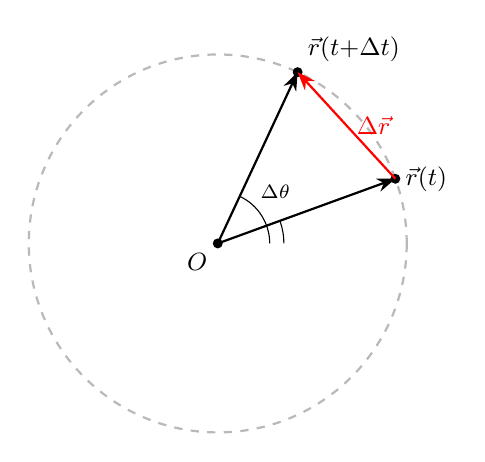
\begin{tikzpicture}[>=Stealth, thick, scale=1.2]
    % Arc
    \draw[dashed, gray!55] (0,0) circle (2);
    \fill (0,0) circle (1.5pt) node[below left, font=\small] {$O$};
    % Two position vectors
    \coordinate (A) at (20:2);
    \coordinate (B) at (65:2);
    \draw[->, thick] (0,0) -- (A) node[right, font=\small] {$\vec{r}(t)$};
    \draw[->, thick] (0,0) -- (B) node[above right, font=\small] {$\vec{r}(t{+}\Delta t)$};
    \fill (A) circle (1.5pt);
    \fill (B) circle (1.5pt);
    % Displacement chord
    \draw[->, thick, red] (A) -- (B) node[midway, right, font=\small] {$\Delta\vec{r}$};
    % Angle arc
    \draw[thin] (0.7,0) arc (0:20:0.7);
    \draw[thin] (0.55,0) arc (0:65:0.55);
    \node[font=\scriptsize] at (42:0.82) {$\Delta\theta$};
\end{tikzpicture}
\caption{Displacement vector $\Delta\vec{r}$ for circular motion over an interval $\Delta t$.}
\label{fig:displacement}
\end{figure}

The magnitude of the displacement is $|\Delta\vec{r}| = 2r\sin(\Delta\theta/2)$. For small angles, $\sin(\Delta\theta/2) \approx \Delta\theta/2$, so
\begin{equation}
    |\Delta\vec{r}| \approx r\,\Delta\theta.
\end{equation}
This is consistent with the limit $\Delta\theta \to 0$, where the chord approaches the arc length $r\,\Delta\theta$. The magnitude of the velocity then follows as
\begin{equation}
    v \equiv |\vec{v}(t)| = \lim_{\Delta t\to 0}\frac{|\Delta\vec{r}|}{\Delta t} = r\lim_{\Delta t\to 0}\frac{\Delta\theta}{\Delta t} = r\frac{d\theta}{dt} = r\omega.
\end{equation}
As $\Delta t\to 0$, the direction of $\Delta\vec{r}$ approaches the tangent to the circle, perpendicular to $\vec{r}(t)$ and in the $+\hat{\theta}$-direction for counterclockwise motion. This confirms that the velocity is always tangent to the circle.

% ==============================================================
\subsection{Tangential and Radial Acceleration}
% ==============================================================

In polar coordinates, the acceleration has two components: a tangential component $a_\theta$ and a radial component $a_r$,
\begin{equation}
    \vec{a}(t) = a_r\,\hat{r}(t) + a_\theta\,\hat{\theta}(t).
\end{equation}
The unit vectors $\hat{r}(t)$ and $\hat{\theta}(t)$ change direction with time and are therefore not constant. To compute the acceleration, we differentiate the velocity $\vec{v}(t) = r(d\theta/dt)\,\hat{\theta}(t)$ using the product rule,
\begin{equation}
    \vec{a}(t) = r\frac{d^2\theta}{dt^2}\,\hat{\theta}(t) + r\frac{d\theta}{dt}\frac{d\hat{\theta}}{dt}.
\end{equation}
Substituting $d\hat{\theta}/dt = -(d\theta/dt)\hat{r}(t)$,
\begin{equation}
    \vec{a}(t) = r\frac{d^2\theta}{dt^2}\,\hat{\theta}(t) - r\left(\frac{d\theta}{dt}\right)^2\hat{r}(t).
\end{equation}
The two components are therefore
\begin{align}
    a_\theta &= r\frac{d^2\theta}{dt^2}, \label{eq:atangential}\\
    a_r      &= -r\left(\frac{d\theta}{dt}\right)^2 = -r\omega^2 < 0. \label{eq:aradial}
\end{align}
Because $a_r < 0$, the radial component $a_r(t) = -r\omega^2\,\hat{r}(t)$ is always directed towards the centre of the circular orbit. This is the centripetal acceleration.

\begin{workedexample}[5.2: Circular Motion Kinematics]
A particle moves in a circle of radius $R$. At $t = 0$ it is on the $x$-axis. The angle with the positive $x$-axis is $\theta(t) = At^3 - Bt$, where $A$ and $B$ are positive constants. Find (a) the velocity vector and (b) the acceleration vector in polar coordinates. At what time is the centripetal acceleration zero?

\noindent\textbf{Solution.}
The derivatives are $d\theta/dt = 3At^2 - B$ and $d^2\theta/dt^2 = 6At$. The velocity vector is
\[
    \vec{v}(t) = R\frac{d\theta}{dt}\,\hat{\theta}(t) = R(3At^2 - B)\,\hat{\theta}(t).
\]
The acceleration vector is
\[
    \vec{a}(t) = R\frac{d^2\theta}{dt^2}\,\hat{\theta}(t) - R\left(\frac{d\theta}{dt}\right)^2\hat{r}(t) = 6RAt\,\hat{\theta}(t) - R(3At^2 - B)^2\hat{r}(t).
\]
The centripetal acceleration is zero when $d\theta/dt = 0$, that is, when
\[
    3At_1^2 - B = 0 \implies t_1 = \sqrt{\frac{B}{3A}}.
\]
\end{workedexample}

% ==============================================================
\subsection{Period and Frequency for Uniform Circular Motion}
% ==============================================================

If the total tangential force on the object is zero, the tangential acceleration vanishes,
\begin{equation}
    a_\theta = 0,
\end{equation}
and the speed remains constant. This is \textit{uniform circular motion}. The acceleration reduces to
\begin{equation}
    \vec{a}_r(t) = -r\omega^2\,\hat{r}(t) \qquad \text{(uniform circular motion)}.
\end{equation}
Because the speed $v = r\omega$ is constant, the time to complete one full revolution, the \textit{period} $T$, is constant. In one period the object travels the circumference $2\pi r$, so
\begin{equation}
    2\pi r = vT \implies T = \frac{2\pi r}{v} = \frac{2\pi r}{r\omega} = \frac{2\pi}{\omega}.
\end{equation}
The \textit{frequency} $f$ is the reciprocal of the period,
\begin{equation}
    f = \frac{1}{T} = \frac{\omega}{2\pi}.
\end{equation}
The SI unit of frequency is the hertz: $[\mathrm{Hz}] = [\mathrm{s}^{-1}]$. The magnitude of the centripetal acceleration can be written in several equivalent forms. Using $v = r\omega$,
\begin{align}
    |a_r| &= r\omega^2, \label{eq:ar1}\\
    |a_r| &= \frac{v^2}{r}, \label{eq:ar2}\\
    |a_r| &= 4\pi^2 r f^2, \label{eq:ar3}\\
    |a_r| &= \frac{4\pi^2 r}{T^2}. \label{eq:ar4}
\end{align}
Which form to use depends on what information is given about the orbit.

% --------------------------------------------------------------
\subsection{Geometric Interpretation of the Radial Acceleration}
% --------------------------------------------------------------

An object in circular orbit is always accelerating towards the centre. The velocity is always tangent to the circle, so its direction is continuously changing as the object moves. Because the velocity changes direction, the acceleration is non-zero even when the speed is constant.

\begin{figure}[ht]
\centering
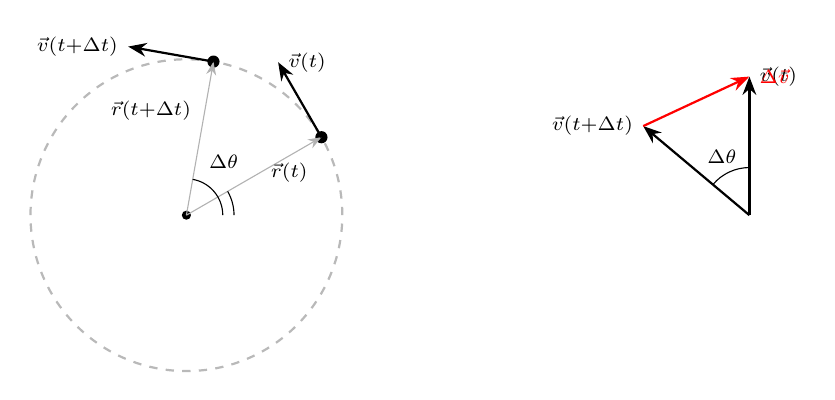
\begin{tikzpicture}[>=Stealth, thick, scale=1.1]
    % Left: circle with two velocity vectors
    \begin{scope}[shift={(-3.5,0)}]
        \draw[dashed, gray!55] (0,0) circle (1.8);
        \fill (0,0) circle (1.5pt);
        % Point at angle 30
        \coordinate (A) at (30:1.8);
        \coordinate (B) at (80:1.8);
        \fill (A) circle (2pt);
        \fill (B) circle (2pt);
        % Position vectors
        \draw[->, thin, gray!60] (0,0) -- (A);
        \draw[->, thin, gray!60] (0,0) -- (B);
        % Velocity at A (tangent, 90 deg CCW)
        \draw[->, thick] (A) -- ++(120:1.0) node[right, font=\scriptsize] {$\vec{v}(t)$};
        % Velocity at B
        \draw[->, thick] (B) -- ++(170:1.0) node[left, font=\scriptsize] {$\vec{v}(t{+}\Delta t)$};
        % Angle label
        \draw[thin] (0.55,0) arc (0:30:0.55);
        \draw[thin] (0.42,0) arc (0:80:0.42);
        \node[font=\scriptsize] at (55:0.75) {$\Delta\theta$};
        % Labels for position vectors
        \node[right, font=\scriptsize] at ($(0,0)!0.55!(A)$) {$\vec{r}(t)$};
        \node[above left, font=\scriptsize] at ($(0,0)!0.55!(B)$) {$\vec{r}(t{+}\Delta t)$};
    \end{scope}
    % Right: velocity triangle
    \begin{scope}[shift={(3.0,0)}]
        % v(t) pointing up
        \coordinate (O2) at (0,0);
        \draw[->, thick] (O2) -- ++(90:1.6) node[right, font=\scriptsize] {$\vec{v}(t)$};
        % v(t+dt) at angle Delta theta from v(t): pointing up-left
        \draw[->, thick] (O2) -- ++(140:1.6) node[left, font=\scriptsize] {$\vec{v}(t{+}\Delta t)$};
        % Delta v (from tip of v(t+dt) to tip of v(t))
        \coordinate (Vtip) at ($(O2)+(90:1.6)$);
        \coordinate (Vdttip) at ($(O2)+(140:1.6)$);
        \draw[->, thick, red] (Vdttip) -- (Vtip) node[right, font=\scriptsize] {$\Delta\vec{v}$};
        % Angle label
        \draw[thin] (0,0.55) arc (90:140:0.55);
        \node[font=\scriptsize] at (115:0.75) {$\Delta\theta$};
    \end{scope}
\end{tikzpicture}
\caption{Left: velocity vectors at two nearby points on a circular orbit. Right: the change in velocity $\Delta\vec{v}$, which points inward as $\Delta\theta\to 0$.}
\label{fig:velchange}
\end{figure}

The magnitude of the change in velocity is $|\Delta\vec{v}| = 2v\sin(\Delta\theta/2) \approx v\,\Delta\theta$ for small $\Delta\theta$ (Figure~\ref{fig:velchange}). The magnitude of the radial acceleration is therefore
\begin{equation}
    |a_r| = \lim_{\Delta t\to 0}\frac{|\Delta\vec{v}|}{\Delta t} = v\lim_{\Delta t\to 0}\frac{\Delta\theta}{\Delta t} = v\frac{d\theta}{dt} = v\omega = \frac{v^2}{r}.
\end{equation}
As $\Delta\theta\to 0$, the direction of $\Delta\vec{v}$ is perpendicular to $\vec{v}$ and directed inward, in the $-\hat{r}$-direction, confirming the centripetal character of the acceleration.

% ==============================================================
\subsection{Angular Velocity and Angular Acceleration}
% ==============================================================

% --------------------------------------------------------------
\subsection{Angular Velocity}
% --------------------------------------------------------------

We always choose a right-handed cylindrical coordinate system. With the positive $z$-axis pointing up, the angle $\theta$ increases counterclockwise as viewed from above. The \textit{angular velocity vector} for a point object undergoing circular motion about the $z$-axis is directed along the $z$-axis,
\begin{equation}
    \vec{\omega} = \frac{d\theta}{dt}\,\hat{k} = \omega_z\,\hat{k}.
\end{equation}
The angular speed is the magnitude of the $z$-component, $\omega \equiv |\omega_z| = |d\theta/dt|$. If the object rotates counterclockwise, $\omega_z = d\theta/dt > 0$ and $\vec{\omega}$ points in the $+\hat{k}$-direction. If the object rotates clockwise, $\omega_z < 0$ and $\vec{\omega}$ points in the $-\hat{k}$-direction.

The velocity and angular velocity are related by the cross product,
\begin{equation}
    \vec{v} = \vec{\omega}\times\vec{r} = \frac{d\theta}{dt}\,\hat{k}\times r\hat{r} = r\frac{d\theta}{dt}\,\hat{\theta}.
\end{equation}

\begin{workedexample}[5.3: Angular Velocity]
A particle moves in a circle of radius $R$. At $t = 0$ it is on the $x$-axis. The angle with the positive $x$-axis is $\theta(t) = At - Bt^3$, where $A$ and $B$ are positive constants. Find (a) the angular velocity vector, (b) the velocity vector, (c) the time $t_1$ when the angular velocity is zero, and (d) the direction of $\vec{\omega}$ for $t < t_1$ and $t > t_1$.

\noindent\textbf{Solution.} The derivative of $\theta(t)$ is
\[
    \frac{d\theta}{dt} = A - 3Bt^2.
\]
(a) The angular velocity vector is
\[
    \vec{\omega}(t) = (A - 3Bt^2)\,\hat{k}.
\]
(b) The velocity is
\[
    \vec{v}(t) = R(A - 3Bt^2)\,\hat{\theta}(t).
\]
(c) The angular velocity is zero when
\[
    A - 3Bt_1^2 = 0 \implies t_1 = \sqrt{\frac{A}{3B}}.
\]
(d) For $t < t_1$, $d\theta/dt > 0$ so $\vec{\omega}$ points in the $+\hat{k}$-direction (counterclockwise). For $t > t_1$, $d\theta/dt < 0$ so $\vec{\omega}$ points in the $-\hat{k}$-direction (clockwise).
\end{workedexample}

% --------------------------------------------------------------
\subsection{Angular Acceleration}
% --------------------------------------------------------------

The \textit{angular acceleration vector} for circular motion about the $z$-axis is
\begin{equation}
    \vec{\alpha} = \frac{d^2\theta}{dt^2}\,\hat{k} = \alpha_z\,\hat{k}.
\end{equation}
The SI units of angular acceleration are $[\mathrm{rad\cdot s^{-2}}]$. There are four combinations of the signs of $\omega_z$ and $\alpha_z$ to consider.

When $\vec{\alpha}$ points in the $+\hat{k}$-direction ($\alpha_z > 0$): (i) if $\omega_z > 0$ (counterclockwise), the object is speeding up counterclockwise; (ii) if $\omega_z < 0$ (clockwise), the object is slowing down.

When $\vec{\alpha}$ points in the $-\hat{k}$-direction ($\alpha_z < 0$): (iii) if $\omega_z > 0$ (counterclockwise), the object is slowing down; (iv) if $\omega_z < 0$ (clockwise), the object is speeding up clockwise.

The tangential and radial components of the acceleration (Eqs.~(\ref{eq:atangential}) and (\ref{eq:aradial})) can be written compactly as $a_\theta = r\alpha_z$ and $a_r = -r\omega_z^2$.

\begin{workedexample}[5.4: Integration and Circular Motion Kinematics]
A point object is constrained to travel in a circle. The $z$-component of the angular acceleration is
\[
    \alpha_z(t) = \begin{cases} b\!\left(1 - \dfrac{t}{t_1}\right), & 0 \leq t \leq t_1, \\[4pt] 0, & t > t_1, \end{cases}
\]
where $b > 0$ has units $\mathrm{rad\cdot s^{-2}}$. (a) Find the angular velocity at $t = t_1$. (b) Through what angle has the object rotated at $t = t_1$?

\noindent\textbf{Solution.} (a) Starting from rest ($\omega_z(0) = 0$), we integrate:
\[
    \omega_z(t_1) = \int_0^{t_1} b\!\left(1 - \frac{t'}{t_1}\right)dt' = b\!\left[t_1 - \frac{t_1}{2}\right] = \frac{bt_1}{2}.
\]

(b) First find $\omega_z(t)$ for $0 \leq t \leq t_1$:
\[
    \omega_z(t) = \int_0^t b\!\left(1 - \frac{t'}{t_1}\right)dt' = b\!\left(t - \frac{t^2}{2t_1}\right).
\]
Then integrate again to find the angle:
\[
    \theta(t_1) - \theta(0) = \int_0^{t_1}\omega_z(t')\,dt' = \int_0^{t_1} b\!\left(t' - \frac{t'^2}{2t_1}\right)dt' = b\!\left[\frac{t_1^2}{2} - \frac{t_1^2}{6}\right] = \frac{bt_1^2}{3}.
\]
\end{workedexample}


\newpage
% ==============================================================
\section{Gravitation: The Moon is Falling}
% ==============================================================

At the start of our circular-motion story we repeated Newton's remark: the
Moon is always \emph{falling} towards the Earth --- otherwise, by the first
law, it would fly off in a straight line. We now have every tool needed to
take that remark seriously, and it leads to one of the greatest
predict-and-check episodes in the history of science. This section retells
it, and asks you to redo Newton's arithmetic yourself.

In 1665 the plague closed Cambridge University, and the 23-year-old Newton
retreated to his family farm at Woolsthorpe. By his own (much later) telling,
watching an apple fall in the garden set him wondering: the Earth's pull
evidently reaches the top of the tallest tree --- might it reach all the way
to the Moon? If so, the Moon's endless circling and the apple's brief drop
would be \emph{the same phenomenon}. No one had ever connected the heavens
and the ground by a single law. The idea is bold; what makes it science is
that it can be checked by a number.

\begin{predictbox}[5.3: Newton's own prediction]
Suppose the Earth's pull weakens with the \emph{square} of the distance from
the Earth's centre --- Newton's guess, partly inspired by how the light of a
lamp dilutes with distance. An apple sits about one Earth radius from the
centre ($R_E \approx 6.37\times10^6$\,m). The Moon sits about
\emph{sixty} Earth radii away. Under the inverse-square guess:
\begin{enumerate}[leftmargin=2em, itemsep=1pt]
  \item How many times weaker should gravity be at the Moon than at the apple?
  \item The apple accelerates at $g = 9.8\;\mathrm{m/s^2}$. Predict the Moon's
        acceleration.
\end{enumerate}
Answer both before reading on --- then we will \emph{measure} the Moon's actual
acceleration, using nothing but the circular-motion formulas you just learned
and two numbers astronomers have known since antiquity.
\end{predictbox}

\subsection{The Moon Test}

If the inverse-square guess is right, gravity at the Moon should be weaker by
a factor of $60^2 = 3600$, so the Moon should be falling with acceleration
\begin{equation*}
    a_{\text{predicted}} = \frac{g}{3600} = \frac{9.8}{3600}
    \approx 2.7\times10^{-3}\;\mathrm{m/s^2}.
\end{equation*}
That is the prediction. Now the check. The Moon moves in a (nearly) circular
orbit, and for circular motion we know exactly what the centripetal
acceleration must be --- Eq.~\eqref{eq:ar4}:
\begin{equation*}
    |a_r| = \frac{4\pi^2 r}{T^2}.
\end{equation*}
The orbital radius is $r = 3.84\times10^8$\,m and the orbital period is
$T = 27.3\;\text{days} = 2.36\times10^6$\,s. Therefore the Moon's actual
acceleration is
\begin{equation*}
    |a_r| = \frac{4\pi^2 (3.84\times10^8)}{(2.36\times10^6)^2}
    \approx 2.7\times10^{-3}\;\mathrm{m/s^2}.
\end{equation*}
The prediction and the measurement agree. Newton, recalling the calculation
years later, wrote that he ``compared the force requisite to keep the Moon in
her orb with the force of gravity at the surface of the earth, and found them
answer pretty nearly.'' \emph{Pretty nearly} --- the understatement of the
seventeenth century. The apple and the Moon fall by the same law, and the
law is inverse-square.

Notice what kind of argument this is: guess a law, extract a numerical
prediction, and confront it with a measurement that had no right to agree by
accident. A factor of 3600, predicted from a hunch about lamplight, confirmed
to within a percent. You will use exactly this pattern --- predict, then
check --- in your own experiments this year, if with slightly smaller stakes.

\subsection{The Law of Universal Gravitation}

Newton generalised the moon test into a law that applies to every pair of
masses in the universe --- two galaxies, or two sesame seeds.

\begin{keybox}[Newton's Law of Universal Gravitation]
Any two point masses $m_1$ and $m_2$ separated by a distance $r$ attract each
other along the line joining them with a force of magnitude
\begin{equation}
    F_g = G\,\frac{m_1 m_2}{r^2},
\end{equation}
where $G$ is the \textbf{universal gravitational constant},
\begin{equation*}
    G = 6.674\times10^{-11}\;\mathrm{N\,m^2\,kg^{-2}}.
\end{equation*}
By the Third Law the two masses feel equal and opposite pulls: the Earth
pulls the apple, and the apple pulls the Earth, with the same force.
\end{keybox}

Two remarks. First, for a sphere (like the Earth) the law applies as if all
the mass were concentrated at the centre --- a theorem that cost Newton real
effort to prove, and part of why he delayed publishing for twenty years.
That is why the apple's distance counts as one Earth \emph{radius}, measured
from the centre, not from the ground. Second, the constant $G$ is
astonishingly small: gravity is by far the weakest force you will meet in
this course. Two 1\,kg masses held 1\,m apart attract with about
$10^{-10}$\,N --- roughly the weight of a single flake of dust. Gravity runs
the universe only because masses like planets are enormous, and because,
unlike electricity, gravity has no negative charge to cancel it.

The value of $G$ was not measured in Newton's lifetime. In 1798 Henry
Cavendish --- a man so shy he communicated with his housekeeper by notes ---
suspended a dumbbell of small lead spheres from a fine wire and measured the
twist produced by the gravitational pull of two larger spheres, a whisper of
a force in a sealed room. Knowing $G$, one can put the Earth itself on the
balance: from $g$ and $R_E$, the Earth's mass follows at once (try the next
example). Cavendish's contemporaries called his experiment ``weighing the
Earth.''

\begin{workedexample}[5.5: Weighing the Earth]
Given $g = 9.81\;\mathrm{m/s^2}$ at the surface, $R_E = 6.37\times10^6$\,m,
and Cavendish's $G$, find the mass of the Earth.

\medskip
\textit{Solution.} A mass $m$ at the surface feels the attraction of the
whole Earth acting from its centre:
\begin{equation*}
    mg = G\,\frac{M_E\,m}{R_E^2}
    \implies M_E = \frac{g R_E^2}{G}
    = \frac{(9.81)(6.37\times10^6)^2}{6.674\times10^{-11}}
    \approx 5.97\times10^{24}\;\mathrm{kg}.
\end{equation*}
Notice that $m$ cancelled: \emph{every} mass at the surface accelerates at
the same $g = GM_E/R_E^2$, which is the deep reason (first noticed by
Galileo) that heavy and light objects fall together. Notice also what the
formula says about altitude: at the International Space Station,
$r = R_E + 400\,\mathrm{km}$, and $g$ drops only to about
$8.7\;\mathrm{m/s^2}$ --- 89\% of its surface value, exactly as Checkpoint
5.1 claimed.
\end{workedexample}

\subsection{Circular Orbits}

For a satellite of mass $m$ in a circular orbit of radius $r$ about the Earth,
gravity is the only force, and it must supply exactly the centripetal
acceleration $v^2/r$ that circular motion demands. Newton's second law in the
radial direction gives
\begin{equation}
    G\,\frac{M_E\,m}{r^2} = \frac{m v^2}{r}
    \implies v = \sqrt{\frac{G M_E}{r}}.
\end{equation}
The satellite's mass cancels again --- a heavy satellite and a paint flake
share any given orbit at the same speed. Writing $v = 2\pi r/T$ and squaring:
\begin{equation}
    T^2 = \frac{4\pi^2}{G M_E}\,r^3. \label{eq:kepler3}
\end{equation}
The square of the period is proportional to the \emph{cube} of the orbital
radius. Keep this result in view; it is about to connect us to an astronomer
who died twelve years before Newton was born.

\subsection{Kepler's Laws}

Between 1576 and 1601, on an island observatory financed by the Danish crown,
Tycho Brahe measured the positions of the planets night after night for
twenty-five years --- the finest naked-eye data ever taken, accurate to about
one-sixtieth of a degree. Johannes Kepler, his difficult and brilliant
assistant, inherited the data and spent nearly a decade in ``war with Mars,''
trying orbit after orbit until the numbers finally surrendered. What they
surrendered to are three laws, published in 1609 and 1619. We state them here;
deriving them fully belongs to a later chapter, but you should know what they
say and where they came from.

\begin{keybox}[Kepler's Laws of Planetary Motion]
\begin{enumerate}[leftmargin=2em, itemsep=2pt]
  \item \textbf{The Law of Ellipses.} Each planet moves on an \emph{ellipse}
        with the Sun at one focus. (A circle is the special case of an
        ellipse with both foci together.)
  \item \textbf{The Law of Equal Areas.} The line from the Sun to a planet
        sweeps out equal areas in equal times --- so a planet moves fastest
        when nearest the Sun and slowest when farthest.
  \item \textbf{The Harmonic Law.} The square of a planet's orbital period is
        proportional to the cube of its mean distance from the Sun:
        $T^2 \propto a^3$, with the \emph{same} constant of proportionality
        for every planet.
\end{enumerate}
\end{keybox}

Kepler found these laws empirically --- pure pattern, no mechanism. He never
knew \emph{why} they were true, though he suspected the Sun. Now look back at
Eq.~\eqref{eq:kepler3}: for circular orbits, the third law fell out of the
law of gravitation in two lines of algebra, complete with the constant
$4\pi^2/GM$ --- the same for every body orbiting the same central mass, just
as Kepler said. (Done with ellipses instead of circles, the same follows
exactly; that computation is beyond us this year.) This was the argument that
convinced Newton's contemporaries: one law, guessed from a falling apple,
reproduced three laws distilled from twenty-five years of Tycho's data. The
second law, the equal-areas rule, has an even prettier origin --- it turns out
to be a disguised conservation law, and it will fall into our hands almost
for free when we meet angular momentum in the next chapter.

\begin{whiteboard}[5.1: The satellite that stands still]
Television dishes in Bhutan point at a fixed spot in the sky. The satellite
they aim at is \emph{geostationary}: it hangs over the same point on the
equator forever.
\begin{enumerate}[label=(\alph*), leftmargin=2.5em, itemsep=1pt]
  \item Before computing: what must such a satellite's orbital period be?
  \item Use Eq.~\eqref{eq:kepler3} to find the orbital radius, and hence the
        altitude above the ground. ($M_E = 5.97\times10^{24}$\,kg; the
        sidereal day is $T = 86\,164$\,s.)
  \item A minister asks for a geostationary satellite parked directly above
        Paro (latitude $27^\circ$N), to improve coverage. As a group, decide:
        is this possible? Defend your answer with the physics of circular
        motion --- where must the centre of any Earth orbit lie?
\end{enumerate}
\textit{(You should find $r \approx 4.2\times10^4$\,km, an altitude of about
36\,000\,km --- a tenth of the way to the Moon. And no: the centre of every
orbit must be the Earth's centre, so a satellite hovering off the equator is
impossible; it would need a circle whose centre is inside northern India.)}
\end{whiteboard}

\begin{supplementary}{The Tides, or: the Sea Breathes Twice a Day}
Bhutan is landlocked, so here is something many of us have never watched: at
the ocean's edge, the water level rises and falls by a metre or more, twice
every day. Newton's law explains this breathing --- and the explanation is
subtler than ``the Moon pulls the water.''

If the Moon simply pulled the water, there would be \emph{one} bulge of ocean
on the Moon's side, and one high tide per day as the Earth turns through it.
The observed rhythm --- two high tides a day --- says otherwise. The key is
that the Moon's pull is \emph{inverse-square}, so it is not uniform across
the Earth: the near-side ocean (about $59\,R_E$ from the Moon) is pulled
harder than the Earth's centre ($60\,R_E$), which in turn is pulled harder
than the far-side ocean ($61\,R_E$). Relative to the Earth, the near water
is pulled ahead, and the Earth is pulled away from the far water. Result:
\emph{two} bulges, one facing the Moon and one facing away, and every coast
passes through both each day. (The Sun pulls far harder in absolute terms,
but tides care about the \emph{difference} in pull across the Earth, and by
that measure the nearby Moon wins --- the Sun's tide is about half the
Moon's. When Sun and Moon line up, at new and full moon, the tides run
extra high.)

How big is the effect? In mid-ocean, under a metre. But geography can
amplify it spectacularly. The world record is the Bay of Fundy in eastern
Canada, where the water rises and falls up to \emph{sixteen metres} --- a
four-storey building, twice daily. The bay is a long, tapering funnel whose
natural sloshing period happens to be close to the 12.4-hour tidal rhythm,
so each tide arrives in step with the bay's own oscillation and pumps it
higher, the way well-timed pushes build up a playground swing. Resonance ---
an idea that will return, from swings to musical instruments to circuits.

Newton's tidal theory, published in the \emph{Principia} in 1687, was the
first time in history the tides had an explanation rather than a mere
timetable. Same law, third appearance: the apple, the Moon, and the sea.
\end{supplementary}

%%-----------Chapter 6------------------------------------------
\chapter{}
 

%% More chapters will be added here as the course progresses.

\end{document}
